\documentclass[12pt,letterpaper]{article}
\usepackage[T1]{fontenc}
\usepackage{lmodern,microtype,amsmath,amssymb,graphicx,booktabs,tabularx,array,enumitem,xcolor,fancyhdr,titlesec,tcolorbox,caption}
\tcbuselibrary{breakable}
\usepackage[margin=1in,headheight=15pt,headsep=18pt,footskip=25pt]{geometry}
\usepackage[colorlinks=true,urlcolor=teal,linkcolor=olive]{hyperref}
\definecolor{olive}{HTML}{536240}\definecolor{ink}{HTML}{293329}\definecolor{teal}{HTML}{17677A}\definecolor{gold}{HTML}{A55C21}\definecolor{soft}{HTML}{EEF3E8}\definecolor{warm}{HTML}{FBEFDF}
\color{ink}\setlength{\parindent}{0pt}\setlength{\parskip}{7pt}
\setlist{leftmargin=1.4em,itemsep=3pt,topsep=3pt}
\renewcommand{\thesection}{1.\arabic{section}}
\titleformat{\section}{\Large\bfseries\color{olive}}{\thesection}{.6em}{}
\titleformat{\subsection}{\large\bfseries\color{teal}}{}{0pt}{}
\titlespacing*{\section}{0pt}{4pt}{12pt}\titlespacing*{\subsection}{0pt}{11pt}{4pt}
\pagestyle{fancy}\fancyhf{}\fancyhead[L]{\small\sffamily MATH\& 107 / WEEK 1}\fancyhead[R]{\small\sffamily Number Systems}\fancyfoot[L]{\small\sffamily Math in Society / Dr Lee}\fancyfoot[R]{\small\sffamily\thepage}\renewcommand{\headrulewidth}{.3pt}
\tcbset{boxrule=.5pt,arc=2mm,left=10pt,right=10pt,top=7pt,bottom=7pt,before skip=9pt,after skip=9pt,colframe=olive!35,colback=soft,fonttitle=\bfseries,coltitle=teal,colbacktitle=soft}
\newcolumntype{Y}{>{\raggedright\arraybackslash}X}
\captionsetup{font=small,labelformat=empty,textfont={color=teal},skip=7pt}
\hypersetup{pdftitle={Week 1: Number Systems},pdfauthor={MATH and 107 / Dr Lee}}
\usepackage{needspace}
\pdfinfoomitdate=1
\pdftrailerid{}
\pdfsuppressptexinfo=15
\setlength{\emergencystretch}{2em}

\widowpenalty=10000
\clubpenalty=10000



\begin{document}
{\small\sffamily\color{olive}WEEK 1 / NUMBER SYSTEMS\par}
\vspace{12pt}
{\fontsize{30}{34}\selectfont\bfseries\color{olive}Counting, movement,\\scaling, and repeated change\par}
\vspace{9pt}
{\large Connect arithmetic to quantities, positions, fractions, and rules that act one step at a time.\par}

\par\medskip\noindent\begin{minipage}{\linewidth}\centering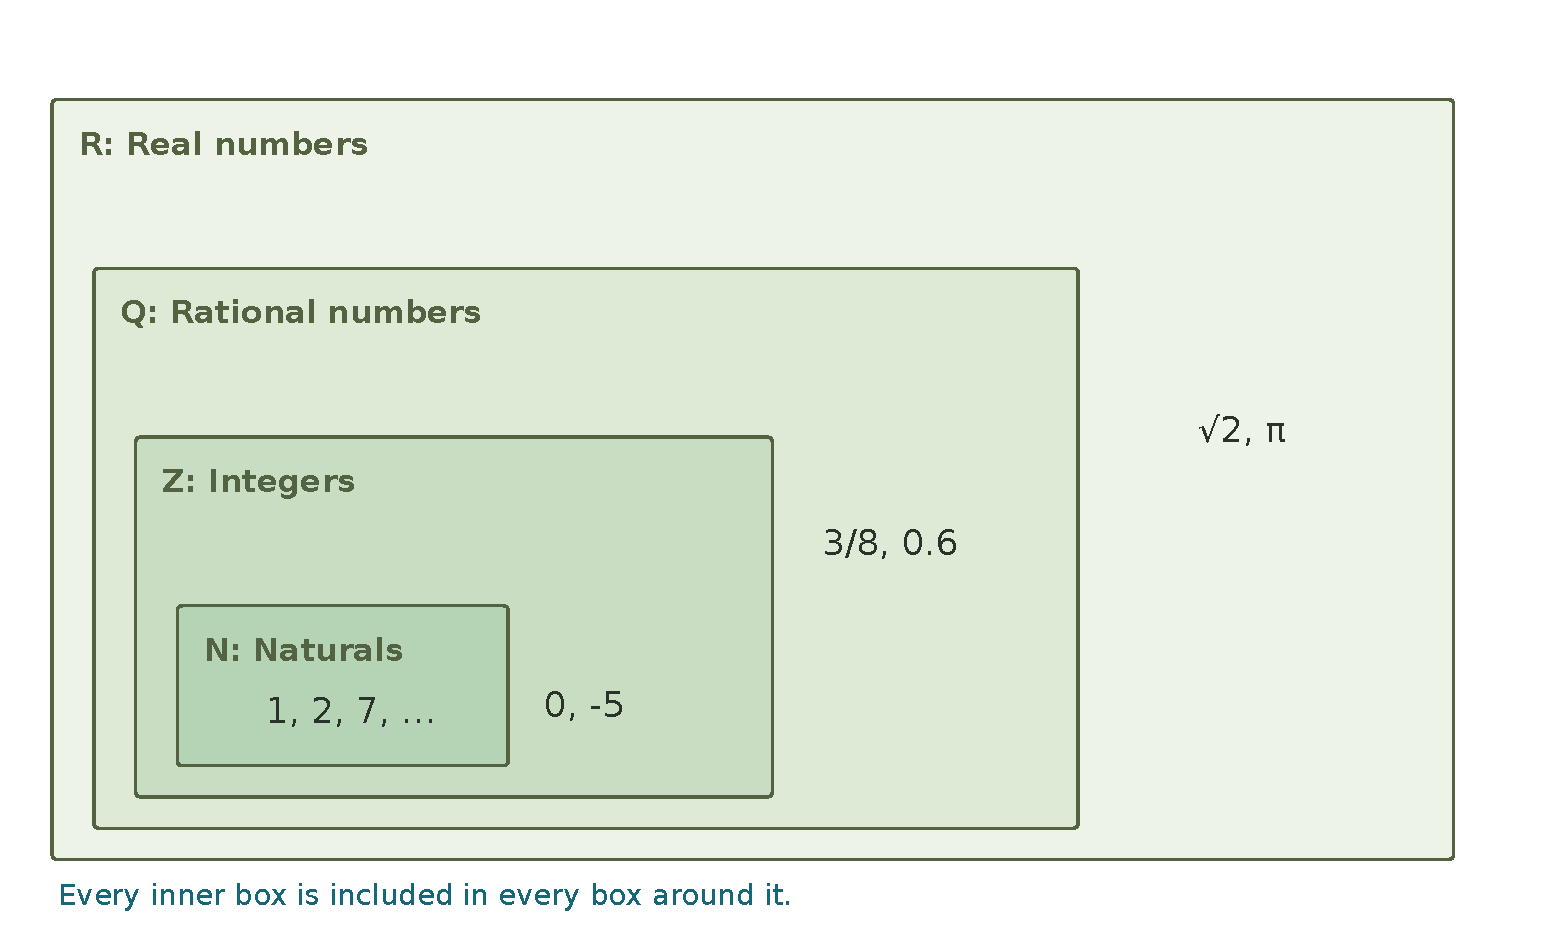
\includegraphics[width=\linewidth,height=2.9in,keepaspectratio]{../assets/week1/number-tower.pdf}\captionof*{figure}{Each smaller system is included in the systems around it. A number can have several correct descriptions.}\end{minipage}\par\medskip

\begin{tcolorbox}[title={Start with what the number means}]
Seven can count books, identify a bus route, mark a temperature, or describe a change. The setting tells us which calculations make sense and what their answers mean.
\end{tcolorbox}
Natural numbers count objects, integers describe signed changes, rational numbers describe ratios, and real numbers locate points on the number line. Repeated additions and multiplications provide two different rules for change.

\medskip
\href{https://bobovski66.github.io/MathInSociety/readings/week1_reading.html}{Online reading}\quad\textperiodcentered\quad\href{https://bobovski66.github.io/MathInSociety/demos/number_systems.html}{Explorer}\quad\textperiodcentered\quad\href{https://bobovski66.github.io/MathInSociety/labs/week1_lab.html}{Laboratory}
\clearpage

\Needspace{6\baselineskip}\section{Quantities, labels, and units}

Seven might be a book count, a bus route, a temperature, or a change in score. The meaning and units determine what we can calculate.


\begin{tcolorbox}[title={What does the number represent?},breakable]

``12'' could mean 12 minutes, 12 dollars, or the label on a storage bin. Adding two waiting times can make sense. Adding the labels on two bins does not tell us how much they contain.


\end{tcolorbox}

A number used as a label identifies something; a number used as a measurement tells us how much of a quantity is present. The distinction matters before any arithmetic begins.


\begin{tcolorbox}[title={Pause and try 1},breakable]
Does ``Bus 8'' mean that the bus contains eight people? What extra information would a count of eight passengers give you?
\end{tcolorbox}

\Needspace{6\baselineskip}\section{The number systems fit inside one another}

A \emph{set} is a collection. The familiar number systems are sets of numbers. We use different names because different situations require different kinds of values.


\par\medskip{\small\renewcommand{\arraystretch}{1.35}\begin{tabularx}{\linewidth}{@{}YYY@{}}\toprule
System & Meaning & Examples\\
\midrule
Natural numbers, \(\mathbb N\) & Positive counting numbers & 1, 2, 3, \ldots{}\\
Integers, \(\mathbb Z\) & Whole numbers, zero, and their negatives & \ldots{}, $-$2, $-$1, 0, 1, 2, \ldots{}\\
Rational numbers, \(\mathbb Q\) & Ratios of integers with a nonzero denominator & 3/8, $-$5/2, 0.6, 7/1\\
Real numbers, \(\mathbb R\) & All positions on the number line, rational or irrational & \(\sqrt2\), \(\pi\), and all the numbers above\\
\bottomrule\end{tabularx}}\par\medskip

Here the natural numbers start at 1. The term \emph{whole numbers} usually means 0, 1, 2, \ldots{} . The classification tasks use the four listed systems, so zero's smallest listed system is the integers.


\par\medskip\noindent\begin{minipage}{\linewidth}
\centering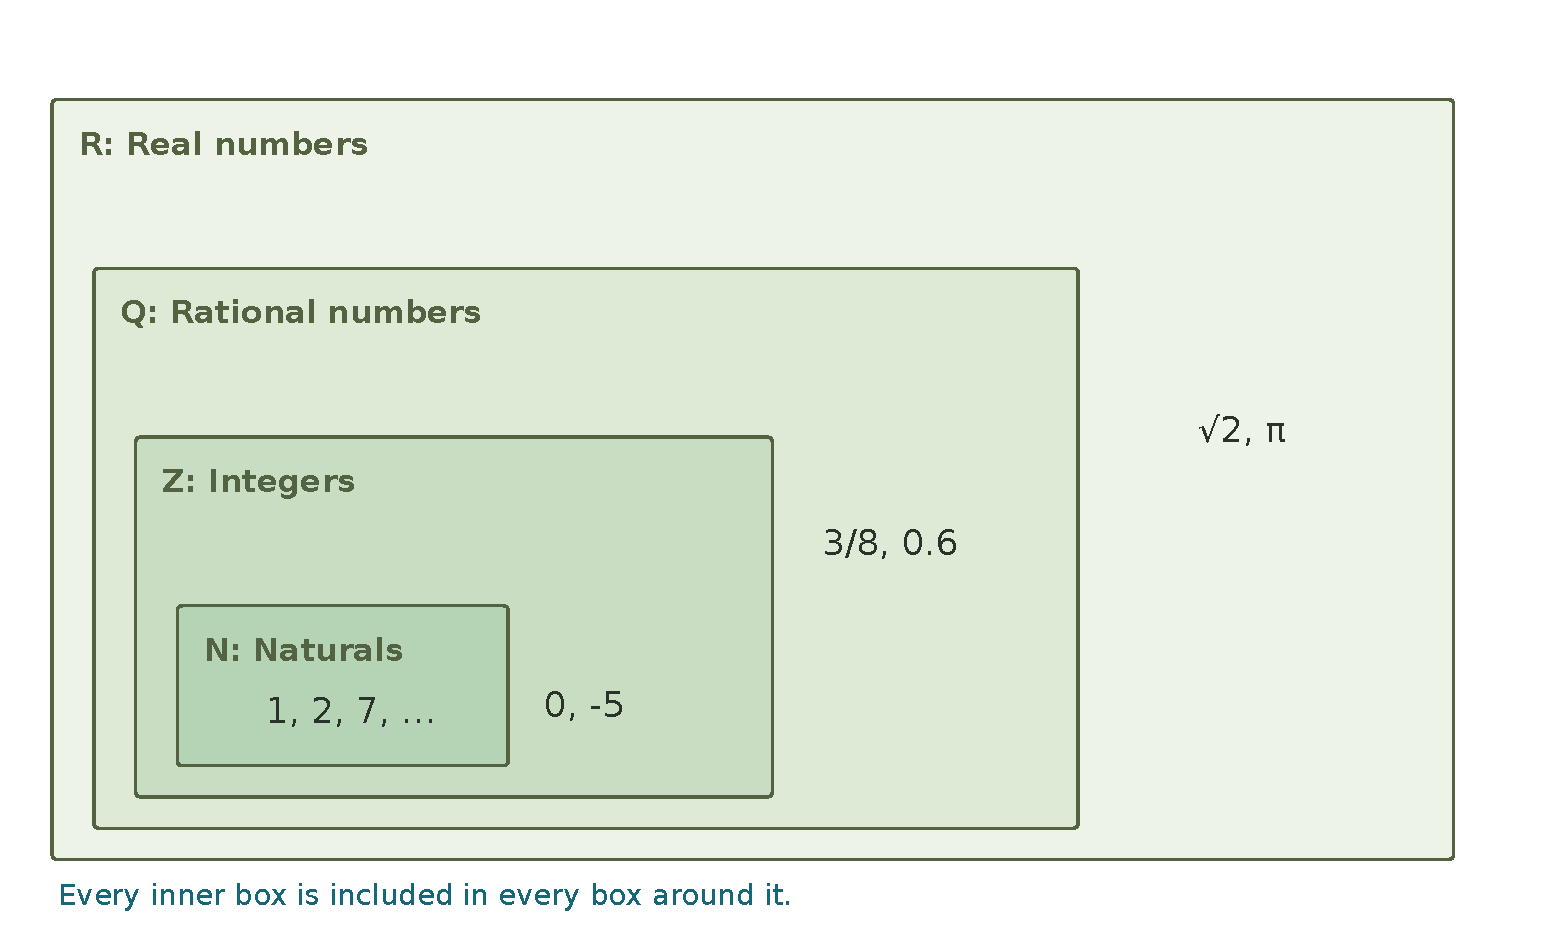
\includegraphics[width=\linewidth,height=3.2in,keepaspectratio]{../assets/week1/number-tower.pdf}
\captionof*{figure}{A natural number is also an integer, a rational number, and a real number.}
\end{minipage}\par\medskip
\[\mathbb N\subset\mathbb Z\subset\mathbb Q\subset\mathbb R.\]
The symbol \(\subset\) means ``is contained in.'' Every integer is rational because it can be written over 1: $-$5 = $-$5/1. Every rational number is real. The fraction 3/8, for example, is rational but is not an integer.


We classify a number by the smallest set in the chain that contains it. For example, \(8/4=2\) is natural, although it is written as a fraction. A value such as \(\sqrt2\) is real but lies outside the rational numbers.


\begin{tcolorbox}[title={Pause and try 2},breakable]
Classify $-$6, 0.25, and 10/2 by their smallest listed systems.
\end{tcolorbox}

\Needspace{6\baselineskip}\section{Addition describes a signed change}

A number line gives zero a location and fixes which direction is positive. On a horizontal line, right is positive and left is negative. A signed change tells us how far to move and which way.


\begin{tcolorbox}[title={Start, then make the change},breakable]

For $-$3 + 5, start at $-$3 and move 5 units right. The end position is 2. For 4 + ($-$7), start at 4 and move 7 units left. The end position is $-$3.


\end{tcolorbox}

\par\medskip\noindent\begin{minipage}{\linewidth}
\centering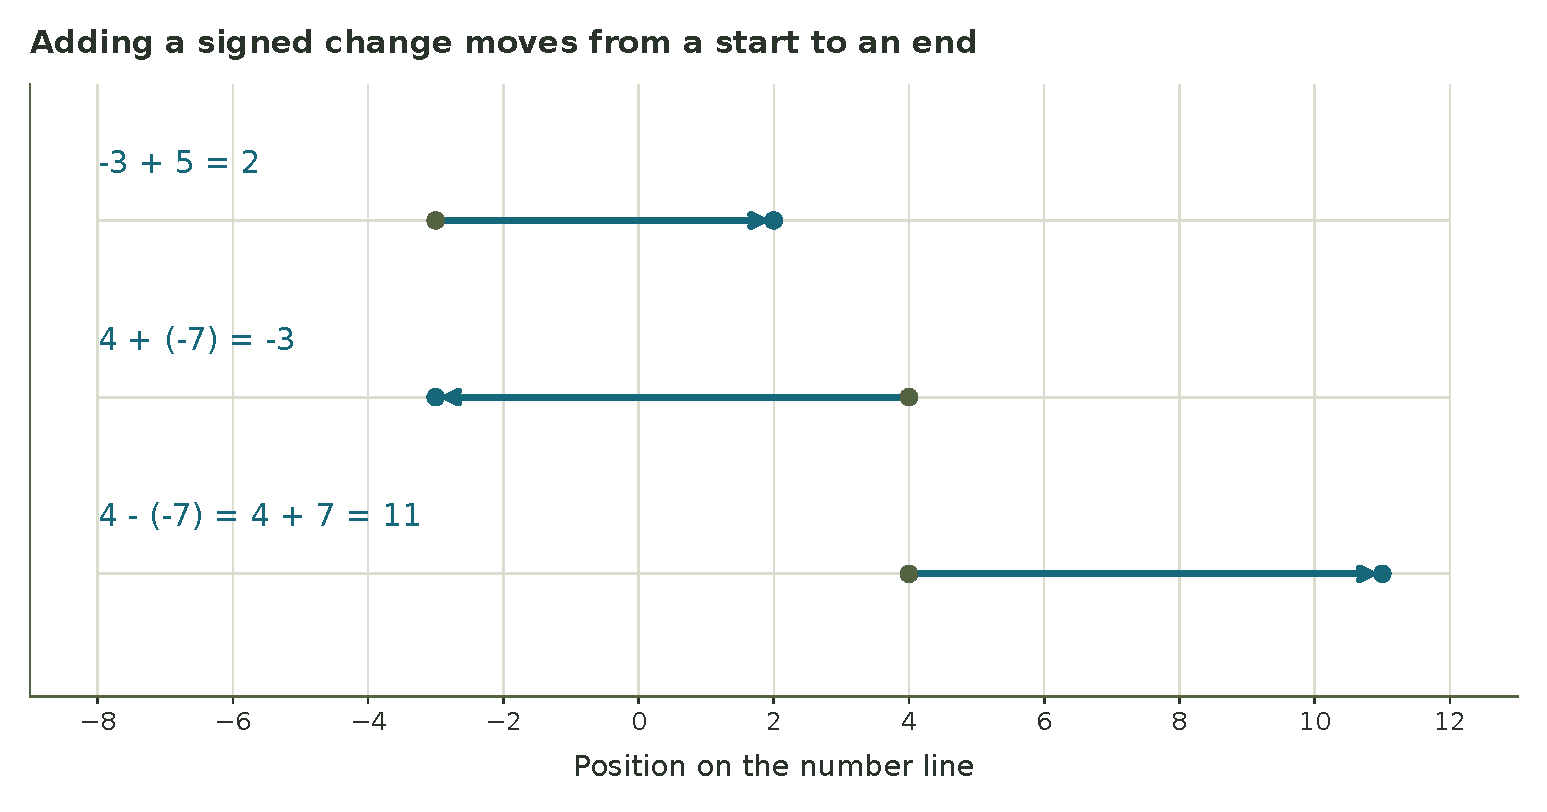
\includegraphics[width=\linewidth,height=2.65in,keepaspectratio]{../assets/week1/signed-motion.pdf}
\captionof*{figure}{The start and the signed change together determine the final position.}
\end{minipage}\par\medskip

Subtracting a number means adding its opposite. Therefore 4 $-$ ($-$7) = 4 + 7 = 11. The minus sign in ``$-$7'' is part of the number being subtracted; taking its opposite gives +7.


Fractions can also describe positions on the number line. To calculate \(1/3+1/2\), express both distances in sixths: \(2/6+3/6=5/6\). The common denominator gives us pieces of the same size.


\begin{tcolorbox}[title={Pause and try 3},breakable]
A submarine is at $-$45 meters relative to the surface and rises 18 meters. Where does it end?
\end{tcolorbox}

\Needspace{6\baselineskip}\section{Position and change}

If a temperature rises from $-$5 to 3 degrees, the final temperature is 3 degrees. The change is +8 degrees. The temperature is 3 degrees; the increase is 8 degrees.


\par\medskip\noindent\begin{minipage}{\linewidth}
\centering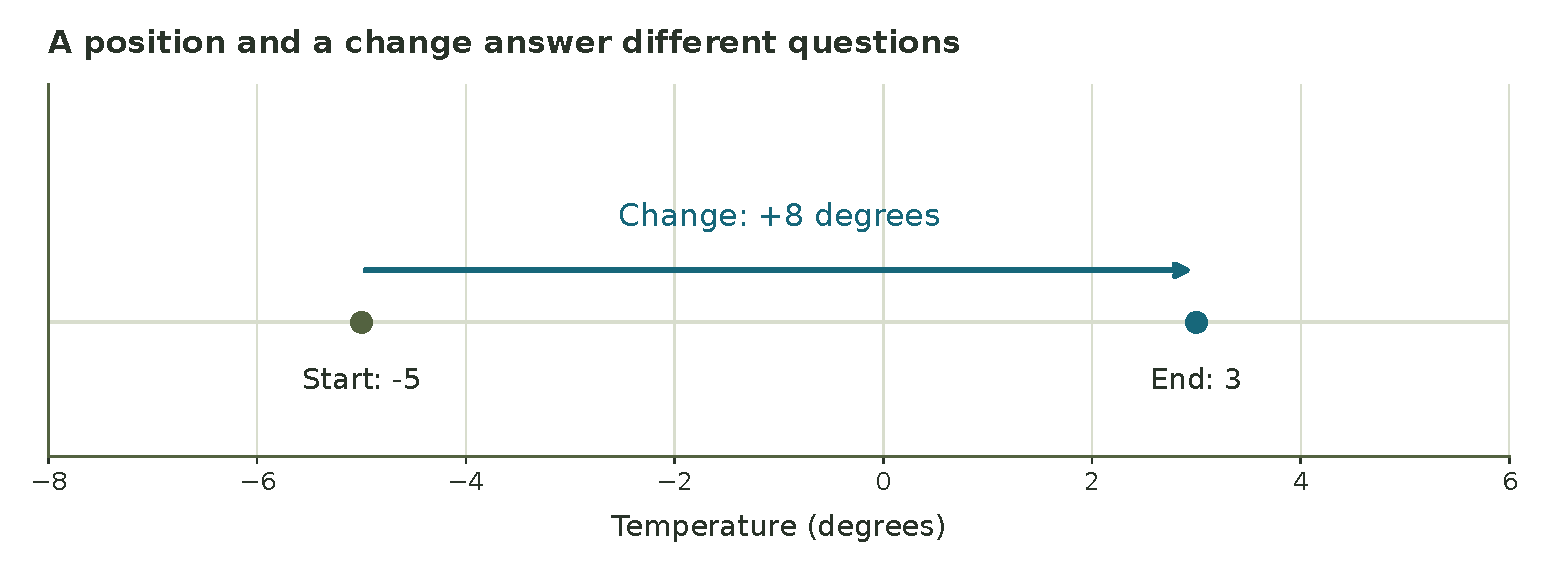
\includegraphics[width=\linewidth,height=2.65in,keepaspectratio]{../assets/week1/position-change.pdf}
\captionof*{figure}{End position = start position + signed change. To recover the change, subtract the start from the end.}
\end{minipage}\par\medskip

\begin{tcolorbox}[title={Follow several changes in order},breakable]

A hiker starts at $-$20 feet relative to sea level, climbs 35 feet, then descends 8 feet. The positions are $-$20, 15, and 7 feet. The final position is 7 feet; the net change from the start is +27 feet.


\end{tcolorbox}

Negative values depend on the choice of units and reference point. A negative elevation can mean below sea level. A negative bank balance can mean an amount owed. A negative count of books on a shelf would usually signal that the chosen model no longer fits the situation.


\begin{tcolorbox}[title={Pause and try 4},breakable]
A game score changes from 14 to 9. What is the change, and how would you write the update?
\end{tcolorbox}

\Needspace{6\baselineskip}\section{Fractions name shares and locations}

In 3/4, the denominator 4 says that one whole is divided into four equal parts. The numerator 3 says to take three of those parts. For a length, 3/4 also marks a position between 0 and 1.


Different fractions can name the same share. Multiply the numerator and denominator by the same nonzero number to keep the value unchanged: 1/2 = 2/4 = 3/6 = 50/100.


\par\medskip\noindent\begin{minipage}{\linewidth}
\centering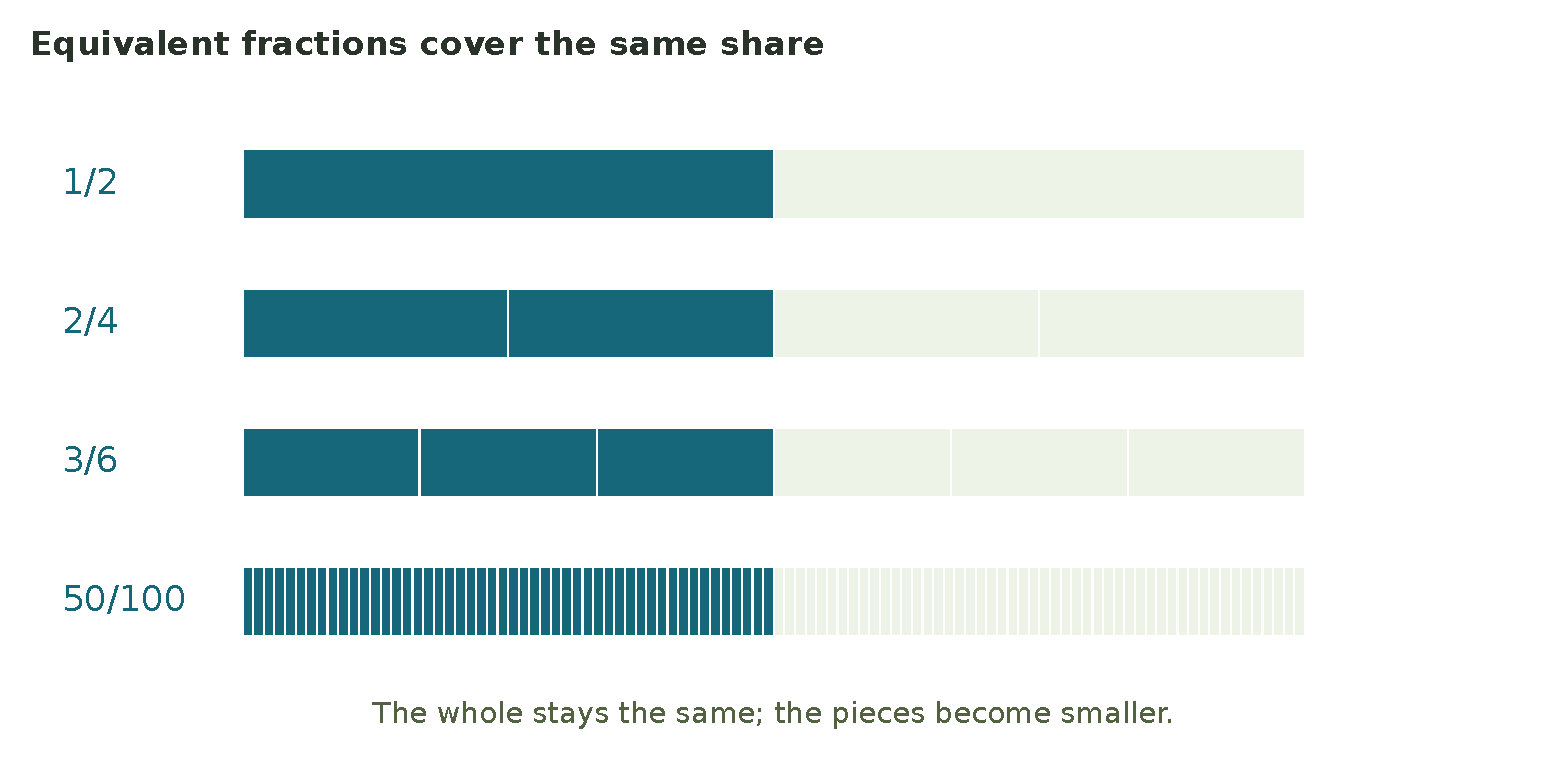
\includegraphics[width=\linewidth,height=2.65in,keepaspectratio]{../assets/week1/fraction-equivalence.pdf}
\captionof*{figure}{The whole has the same size in every row. More pieces does not necessarily mean a larger amount.}
\end{minipage}\par\medskip

\begin{tcolorbox}[title={Two ways to check equivalence},breakable]

3/4 and 9/12 are equal because both numerator and denominator were multiplied by 3. You can also cross-multiply: 3 $\times$ 12 = 36 and 4 $\times$ 9 = 36.


For 2/5 and 7/15, the cross-products are 2 $\times$ 15 = 30 and 5 $\times$ 7 = 35. They are different values.


\end{tcolorbox}

In symbols, a/b = c/d exactly when ad = bc, provided b and d are nonzero. Division by zero is undefined. To simplify 18/24, divide both parts by their greatest common factor, 6: the result is 3/4.


A decimal is another way to write a share. 0.6 means six tenths, so 0.6 = 6/10 = 3/5. A percentage uses hundredths: 0.6 = 60/100 = 60\%.


\begin{tcolorbox}[title={Pause and try 5},breakable]
Are 6/10 and 9/15 equivalent? Show one check.
\end{tcolorbox}

\Needspace{6\baselineskip}\section{Adding, multiplying, and dividing fractions}

To add fractions, first express them in the same-sized pieces. One third and one fourth are different units; twelfths let us count both together.

\[\frac13+\frac14=\frac4{12}+\frac3{12}=\frac7{12}.\]
\par\medskip\noindent\begin{minipage}{\linewidth}
\centering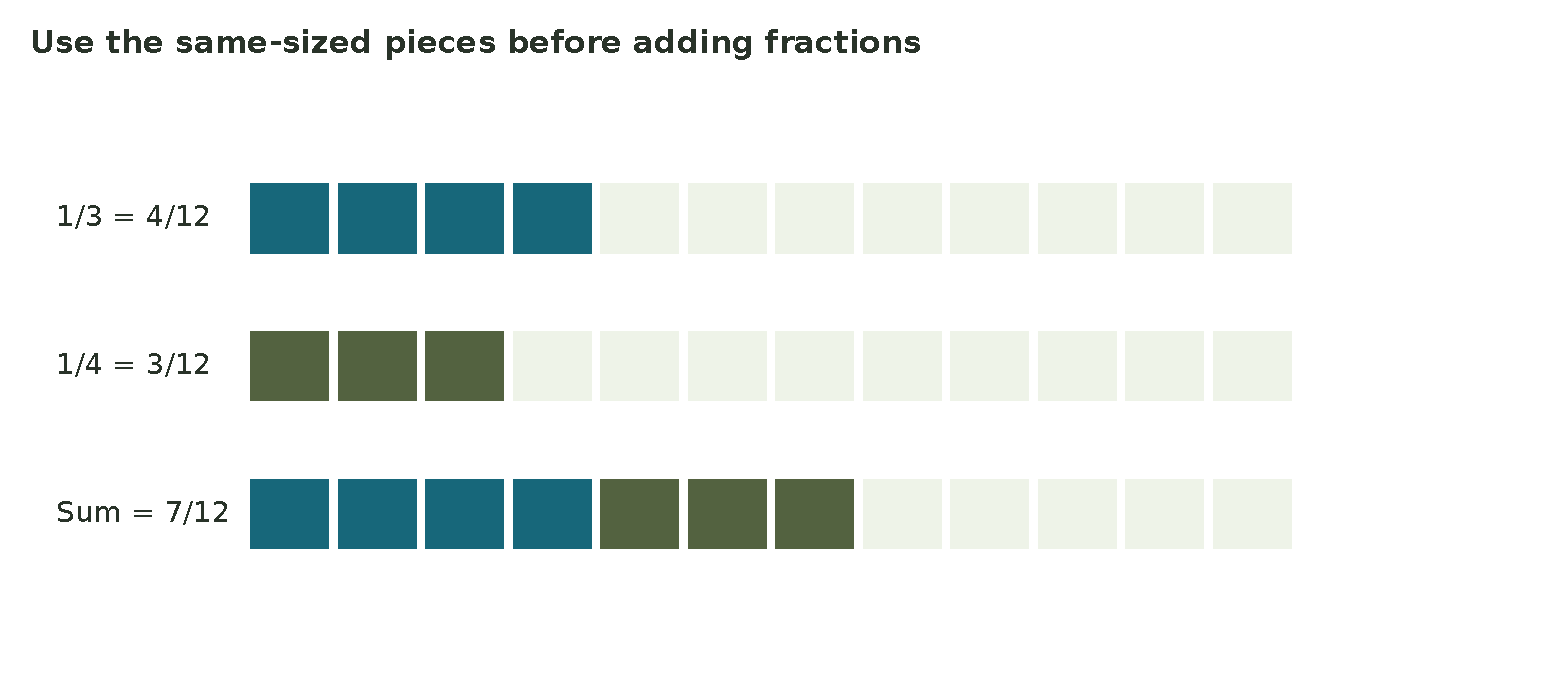
\includegraphics[width=\linewidth,height=2.65in,keepaspectratio]{../assets/week1/common-denominator.pdf}
\captionof*{figure}{Once the pieces have the same size, add their numerators.}
\end{minipage}\par\medskip

Multiplication finds a fraction of an amount. Taking two thirds of a recipe that uses three quarters of a cup means multiplying the two fractions.


\par\medskip\noindent\begin{minipage}{\linewidth}
\centering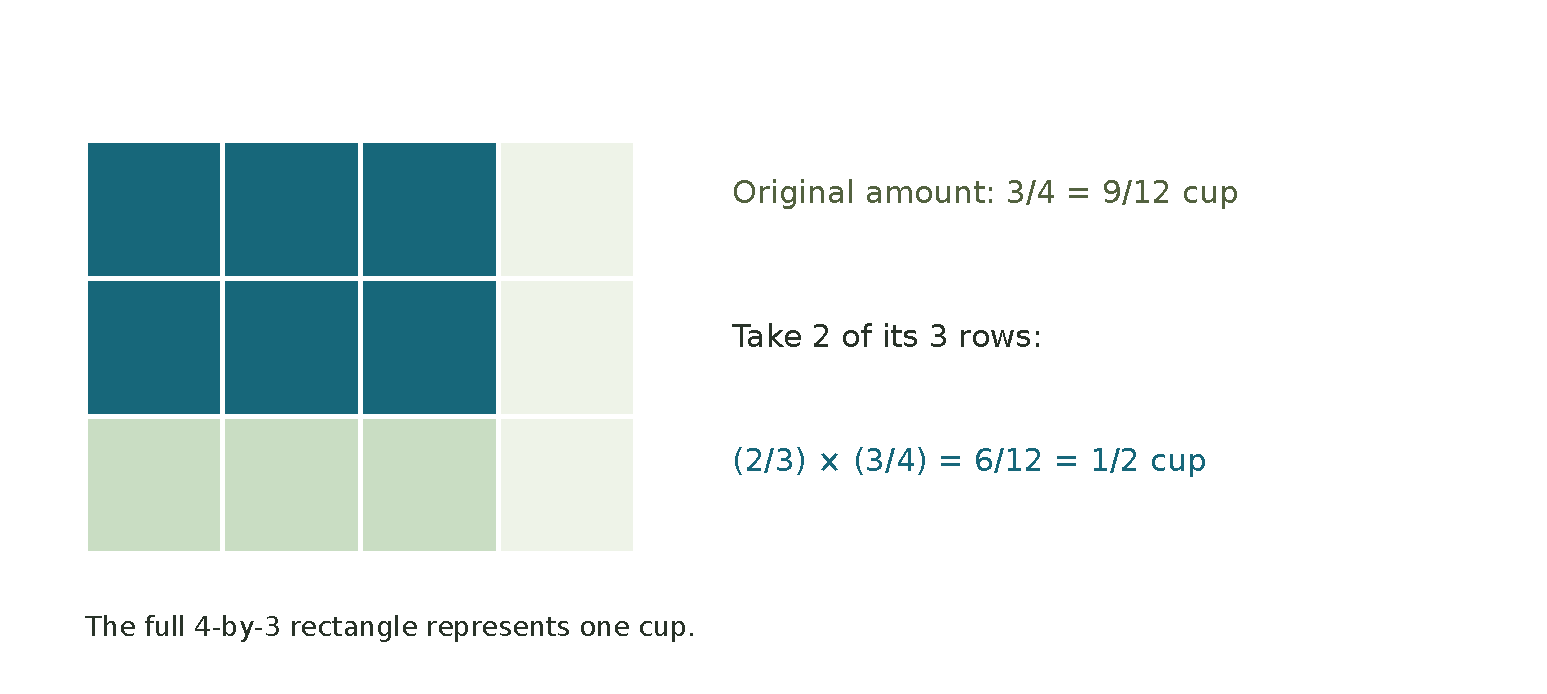
\includegraphics[width=\linewidth,height=2.65in,keepaspectratio]{../assets/week1/fraction-scale.pdf}
\captionof*{figure}{Multiply numerators and denominators: (2/3)(3/4) = 6/12 = 1/2.}
\end{minipage}\par\medskip

Division can count portions. If each portion is 1/3 cup, how many fit into 6 cups? There are three thirds in each cup, giving 18 portions.


\par\medskip\noindent\begin{minipage}{\linewidth}
\centering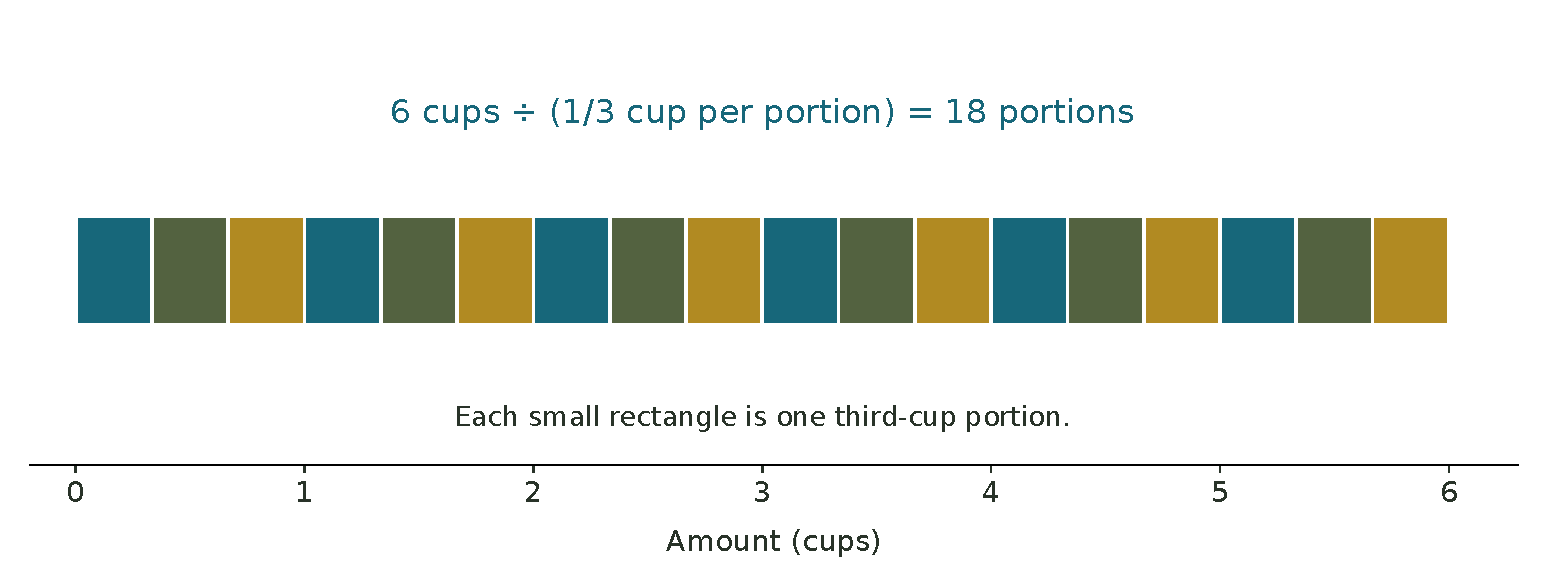
\includegraphics[width=\linewidth,height=2.65in,keepaspectratio]{../assets/week1/division-portions.pdf}
\captionof*{figure}{6 $\div$ (1/3) = 6 $\times$ 3 = 18. Dividing by a small positive fraction can produce a larger number.}
\end{minipage}\par\medskip

In general, dividing by a nonzero number is multiplying by its reciprocal. The reciprocal of 2/3 is 3/2 because their product is 1. For example, (5/6) $\div$ (1/3) = (5/6) $\times$ 3 = 5/2.


\begin{tcolorbox}[title={Pause and try 6},breakable]
Find 1/2 + 1/4 and (1/2) $\times$ (1/4). Why are the results different?
\end{tcolorbox}

\Needspace{6\baselineskip}\section{Multiplication describes a scale factor}

A factor tells us how a value is scaled. Multiplying a positive amount by 2 doubles it. Multiplying by 1/2 halves it. The factor determines whether the distance from zero increases or decreases.


\par\medskip\noindent\begin{minipage}{\linewidth}
\centering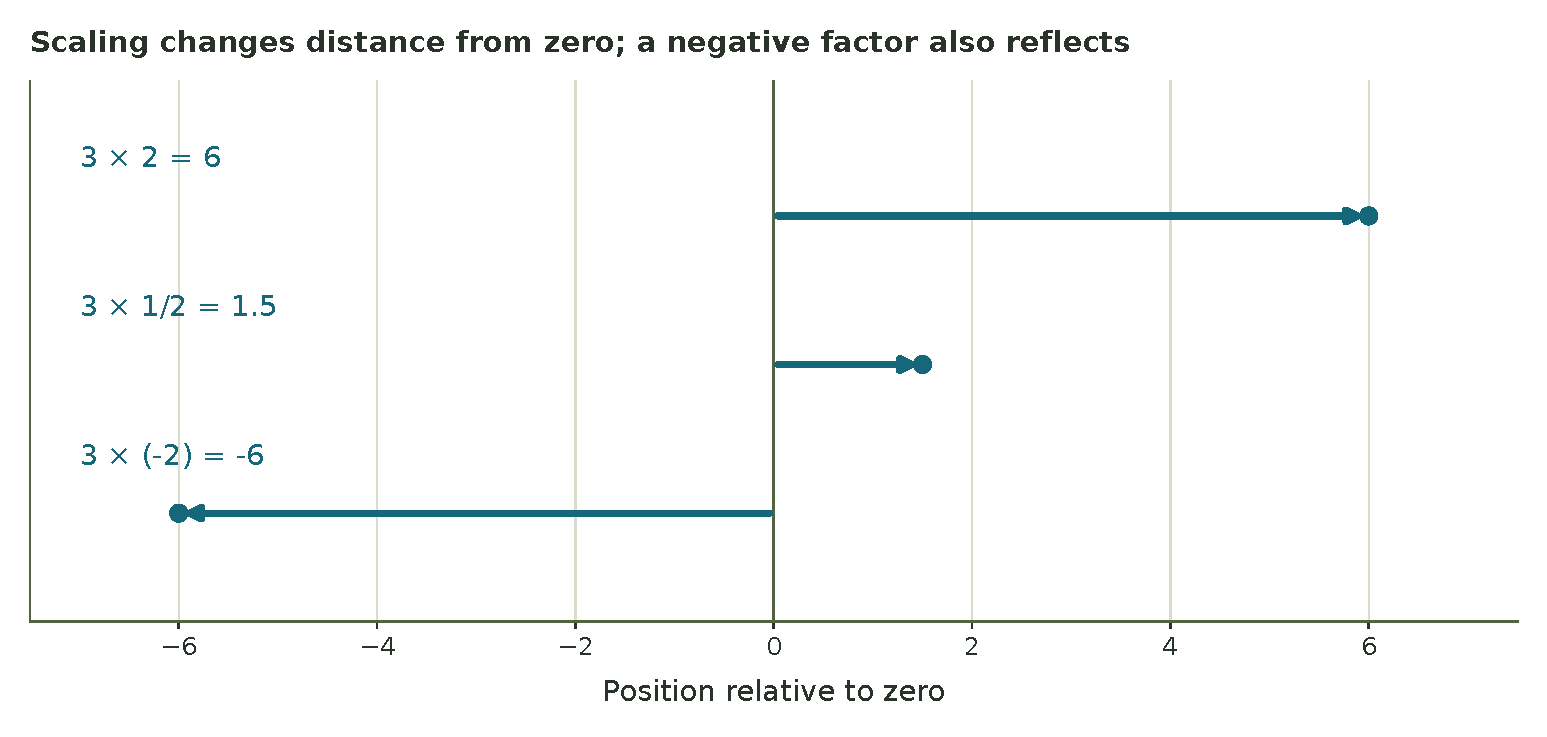
\includegraphics[width=\linewidth,height=2.65in,keepaspectratio]{../assets/week1/scale-factors.pdf}
\captionof*{figure}{For a nonzero value, a factor's absolute size changes distance from zero. A negative factor also changes the side of zero.}
\end{minipage}\par\medskip

For a positive amount, a factor greater than 1 makes it larger; a factor between 0 and 1 makes it smaller; 1 leaves it unchanged; 0 gives zero. A negative factor reflects across zero while scaling the distance.


\begin{tcolorbox}[title={Two negative signs as two reversals},breakable]

Multiplying by $-$1 reflects a point across zero. Applying that reflection twice returns to the original side, so ($-$1)($-$1) = 1. In ($-$2)($-$5) = 10, the negative value is scaled by 5 and reflected again.


\end{tcolorbox}

For a negative start, multiplying by 2 moves farther from zero but lower on the number line: $-$4 $\times$ 2 = $-$8. The growth comparison above assumes a positive amount.


\begin{tcolorbox}[title={Pause and try 7},breakable]
Without calculating exact results, compare 9 $\times$ (1/3) and 9 $\div$ (1/3) with 9.
\end{tcolorbox}

\Needspace{6\baselineskip}\section{A percentage change becomes a multiplier}

Percent means ``per hundred.'' A 10\% increase keeps the original 100\% and adds another 10\%, giving 110\% = 1.10 times the old amount. A 10\% decrease keeps 90\%, so its factor is 0.90.

\[\text{increase factor}=1+\frac{p}{100},\qquad\text{decrease factor}=1-\frac{p}{100}.\]
Use p = 10 for 10\%, or a multiplier of 1.06 for a 6\% increase.


\par\medskip\noindent\begin{minipage}{\linewidth}
\centering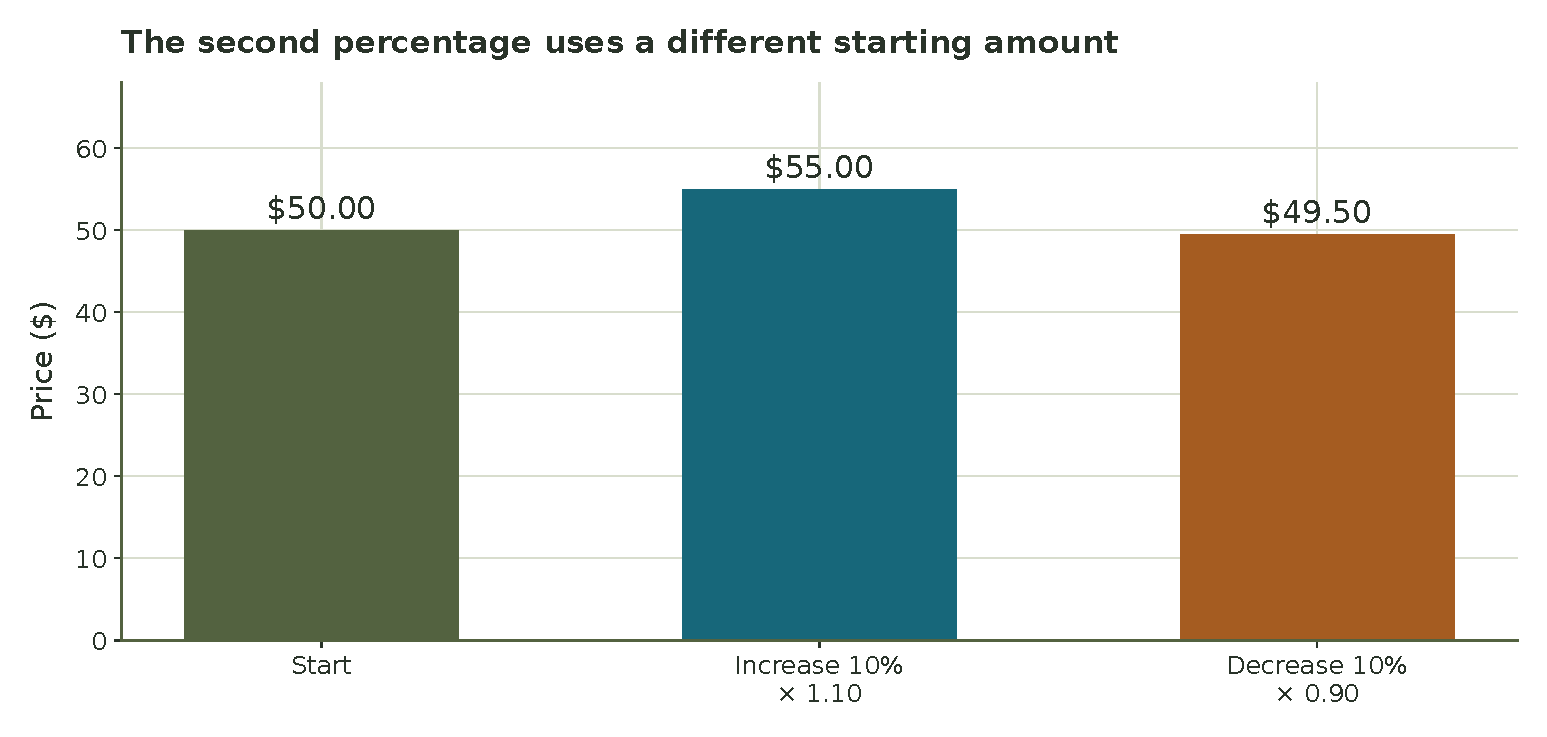
\includegraphics[width=\linewidth,height=2.65in,keepaspectratio]{../assets/week1/percent-round-trip.pdf}
\captionof*{figure}{The second change is calculated from 55 dollars.}
\end{minipage}\par\medskip

Adding a fixed amount and applying a fixed percentage can agree for one step and then differ. Starting at 100, adding 20 gives 120, 140, 160. Growing by 20\% gives 120, 144, 172.80, because each new 20\% is taken from the current amount.


\begin{tcolorbox}[title={Pause and try 8},breakable]
A quantity of 80 increases by 25\%. What factor applies, and what is the new quantity?
\end{tcolorbox}

\Needspace{6\baselineskip}\section{Powers, square roots, and the order of operations}

A power records repeated multiplication. The expression 3$^2$ means 3 $\times$ 3, while 3$^3$ means 3 $\times$ 3 $\times$ 3. The small raised number is an \emph{exponent}. It counts how many copies of the base are multiplied.


The square-root sign asks for the nonnegative number whose square gives the number inside. Thus \(\sqrt{9}\) = 3, \(\sqrt{0}\) = 0, and \(\sqrt{1/4}\) = 1/2.


\par\medskip\noindent\begin{minipage}{\linewidth}
\centering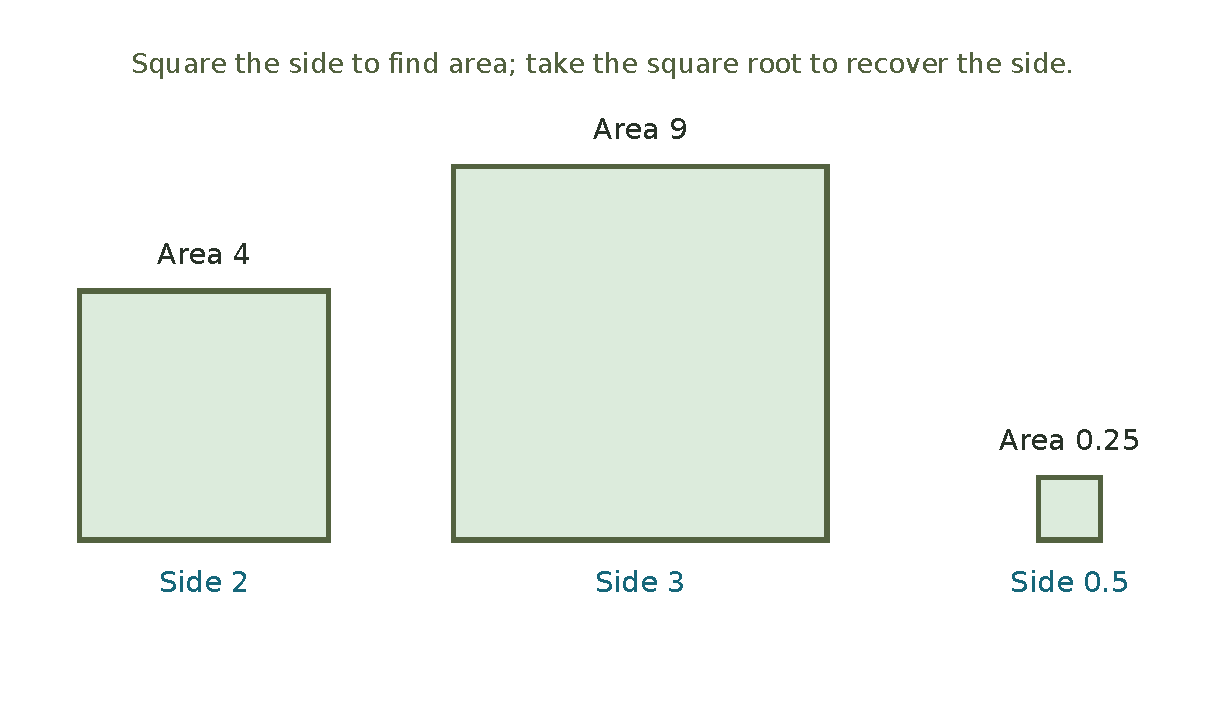
\includegraphics[width=\linewidth,height=2.65in,keepaspectratio]{../assets/week1/powers-and-roots.pdf}
\captionof*{figure}{For example, the square root of 1/4 is 1/2.}
\end{minipage}\par\medskip

\begin{tcolorbox}[title={Keep the sign and the grouping visible},breakable]

($-$4)$^2$ = ($-$4)($-$4) = 16, and \(\sqrt{16}\) = 4. Both 4 and $-$4 solve x$^2$ = 16, but the symbol \(\sqrt{16}\) names only the nonnegative choice.


Compute 2 + 3 $\times$ 4 by multiplying first: 2 + 12 = 14. With parentheses, (2 + 3) $\times$ 4 = 5 $\times$ 4 = 20.


\end{tcolorbox}

Work inside grouping symbols first, then evaluate powers and roots, then multiplication and division from left to right, then addition and subtraction from left to right. A fraction bar also groups its numerator and denominator.


The distributive property says a(b + c) = ab + ac. If a movie club charges 12 dollars plus 4 dollars per visit, the cost for n visits is 12 + 4n. Three people each making n visits pay 3(12 + 4n) = 36 + 12n dollars in all.


\begin{tcolorbox}[title={Pause and try 9},breakable]
Evaluate 3(2 + 5) and 3 $\times$ 2 + 3 $\times$ 5. Then find \(\sqrt{(-3)^2}\).
\end{tcolorbox}

\Needspace{6\baselineskip}\section{An exact number and a decimal approximation differ}

A rational number can be written as a ratio of integers. Its decimal ends or eventually repeats a block: 3/4 = 0.75, while 1/3 = 0.333\ldots{} with the 3 repeating forever.


An \emph{irrational} number is real but cannot be written as a ratio of integers. Its decimal never ends and never settles into a repeating block. \(\sqrt{2}\) and \(\pi\) are examples.


\par\medskip\noindent\begin{minipage}{\linewidth}
\centering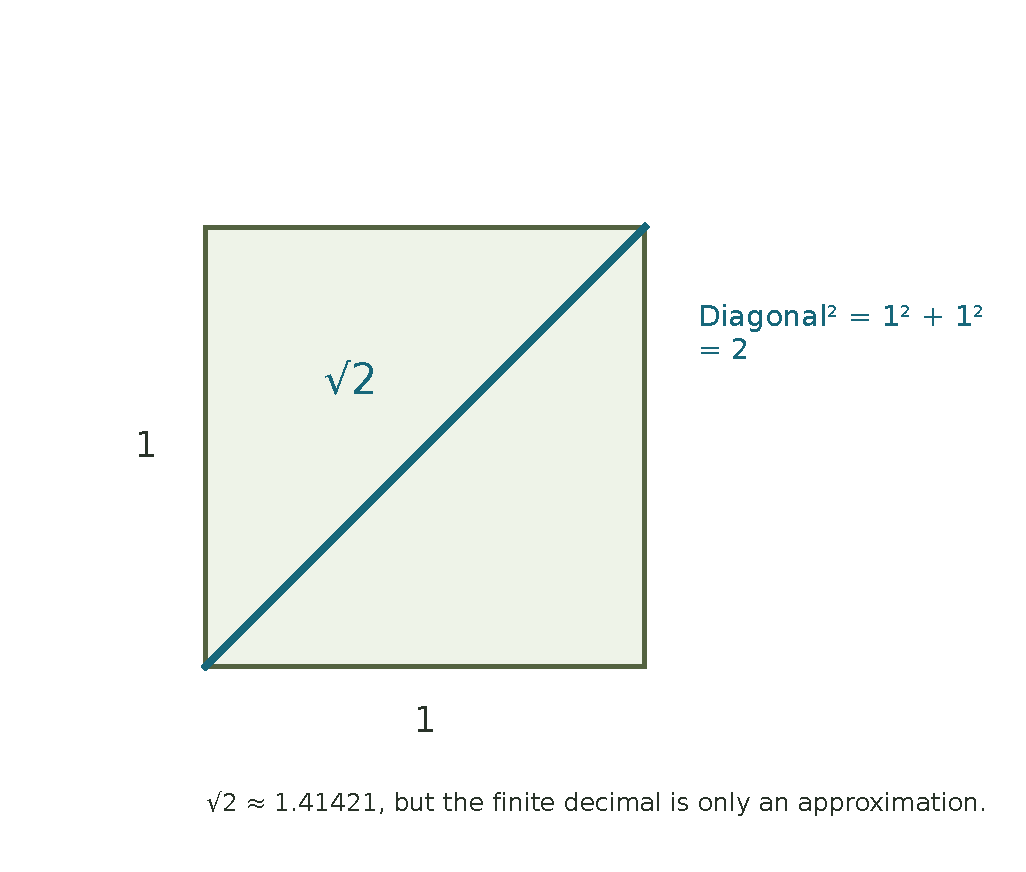
\includegraphics[width=\linewidth,height=3.0in,keepaspectratio]{../assets/week1/unit-square-diagonal.pdf}
\captionof*{figure}{The diagonal has an exact length even though no finite decimal writes that length exactly.}
\end{minipage}\par\medskip

For a nonnegative integer, its square root is rational exactly when the integer is a perfect square, such as 0, 1, 4, 9, or 16. The qualification ``integer'' matters: \(\sqrt{1/4}\) is rational too.


\begin{tcolorbox}[title={Exact values and calculator displays},breakable]

\(\sqrt{2}\) $\approx$ 1.41421. The sign $\approx$ means ``approximately equal.'' The finite decimal 1.41421 is rational; it is not exactly \(\sqrt{2}\). The exact value determines whether a number is rational or irrational.


\end{tcolorbox}

\begin{tcolorbox}[title={Pause and try 10},breakable]
Are \(\sqrt{25}\) and \(\sqrt{6}\) rational or irrational? Is the finite decimal 2.44949 irrational?
\end{tcolorbox}

\Needspace{6\baselineskip}\section{A glimpse beyond the real number line}

No real number squares to $-$1: the square of a real number is never negative. The \emph{complex numbers} extend the real numbers by introducing i, with i$^2$ = $-$1.


A number such as 3 + 2i has two parts. We can draw it at the point (3,2): three units along the real direction and two along the imaginary direction. The vertical axis is called the imaginary axis.


\par\medskip\noindent\begin{minipage}{\linewidth}
\centering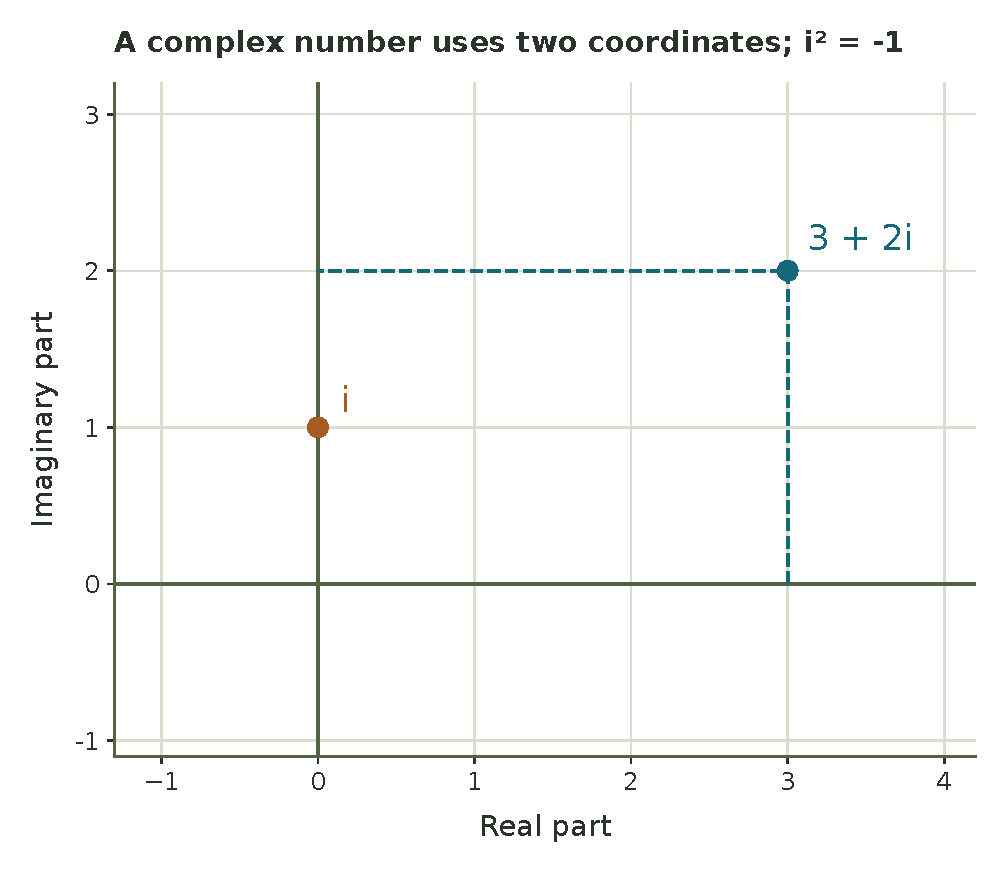
\includegraphics[width=\linewidth,height=3.0in,keepaspectratio]{../assets/week1/complex-plane.pdf}
\captionof*{figure}{Real numbers lie on the horizontal axis. Complex numbers allow points elsewhere in the plane.}
\end{minipage}\par\medskip

This extends the tower to \(\mathbb R\subset\mathbb C\), where \(\mathbb C\) denotes the complex numbers. The classification tasks in this week's assignments use the four real-number systems introduced above.


\begin{tcolorbox}[title={Pause and try 11},breakable]
What are the real and imaginary parts of 5 $-$ 2i?
\end{tcolorbox}

\Needspace{6\baselineskip}\section{Recursion: use the current value to find the next}

A \emph{sequence} is an ordered list. A \emph{recursive rule} tells us how to make a new term from an earlier one. We need both a starting value and an update rule.


\begin{tcolorbox}[title={Starting from a recursive rule},breakable]

Let \(a_0\) = 4 and \(a_{n+1}\) = \(a_n\) + 3. The small numbers are step labels. \(a_0\) means the starting value, \(a_1\) the value after one update, and \(a_2\) the value after two updates. The expression n + 1 means the next step after n.


The rule says: take the current value and add 3. Starting from 4 gives 4, 7, 10, 13, 16, 19.


\end{tcolorbox}

\par\medskip{\small\renewcommand{\arraystretch}{1.35}\begin{tabularx}{\linewidth}{@{}YYY@{}}\toprule
Step n & Add 3 each step & Multiply by 1.5 each step\\
\midrule
0 & 4 & 4\\
1 & 7 & 6\\
2 & 10 & 9\\
3 & 13 & 13.5\\
4 & 16 & 20.25\\
5 & 19 & 30.375\\
\bottomrule\end{tabularx}}\par\medskip

In the second column, the difference between consecutive values stays at 3. In the third, the ratio stays at 1.5. Both start at step 0, before any updates have happened.


\par\medskip\noindent\begin{minipage}{\linewidth}
\centering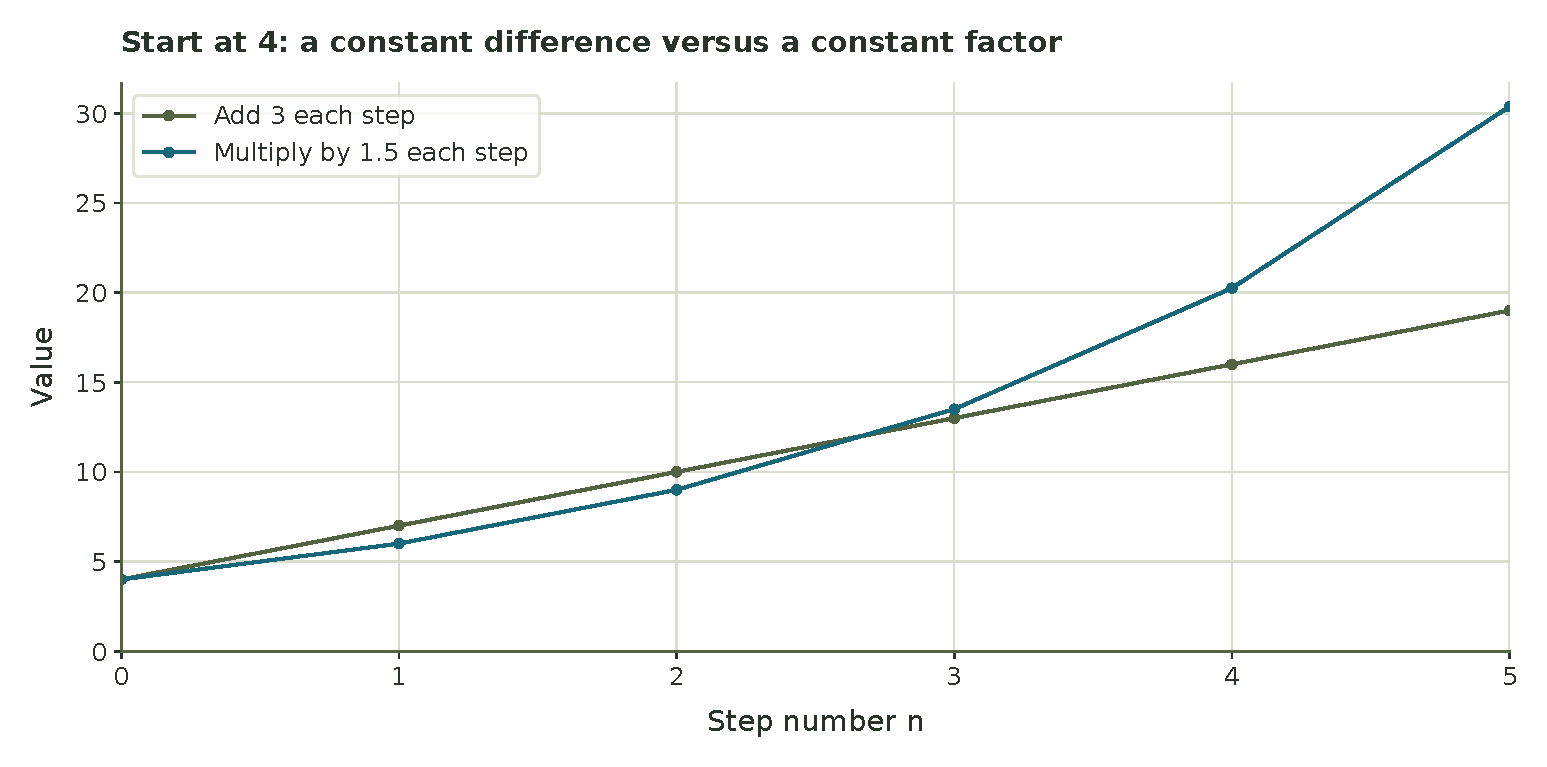
\includegraphics[width=\linewidth,height=2.65in,keepaspectratio]{../assets/week1/recursion-steps.pdf}
\captionof*{figure}{The horizontal axis shows the step number; the vertical axis shows the sequence value.}
\end{minipage}\par\medskip

A \emph{direct formula} can jump to a particular step. With start \(a_0\) and fixed addition d, \(a_n\) = \(a_0\) + nd. With start \(b_0\) and fixed factor r, \(b_n\) = \(b_0\)\(r^n\). The exponent n counts the multiplications; the subscript n labels the term.


For the examples above, \(a_5\) = 4 + 5(3) = 19 and \(b_5\) = 4(1.5)$^5$ = 30.375. A table, a recursive rule, and a direct formula describe the same sequence in different ways.


\begin{tcolorbox}[title={Pause and try 12},breakable]
Start at 9 and subtract 2 at each update. List the start and four updates. What is the step-4 value?
\end{tcolorbox}

\Needspace{6\baselineskip}\section{What repeated rules can describe}

Repeated multiplication can produce growth, decay, or alternating signs. A factor of 1/2 gives decay; a factor of $-$1/2 also reverses the sign each time.


\par\medskip\noindent\begin{minipage}{\linewidth}
\centering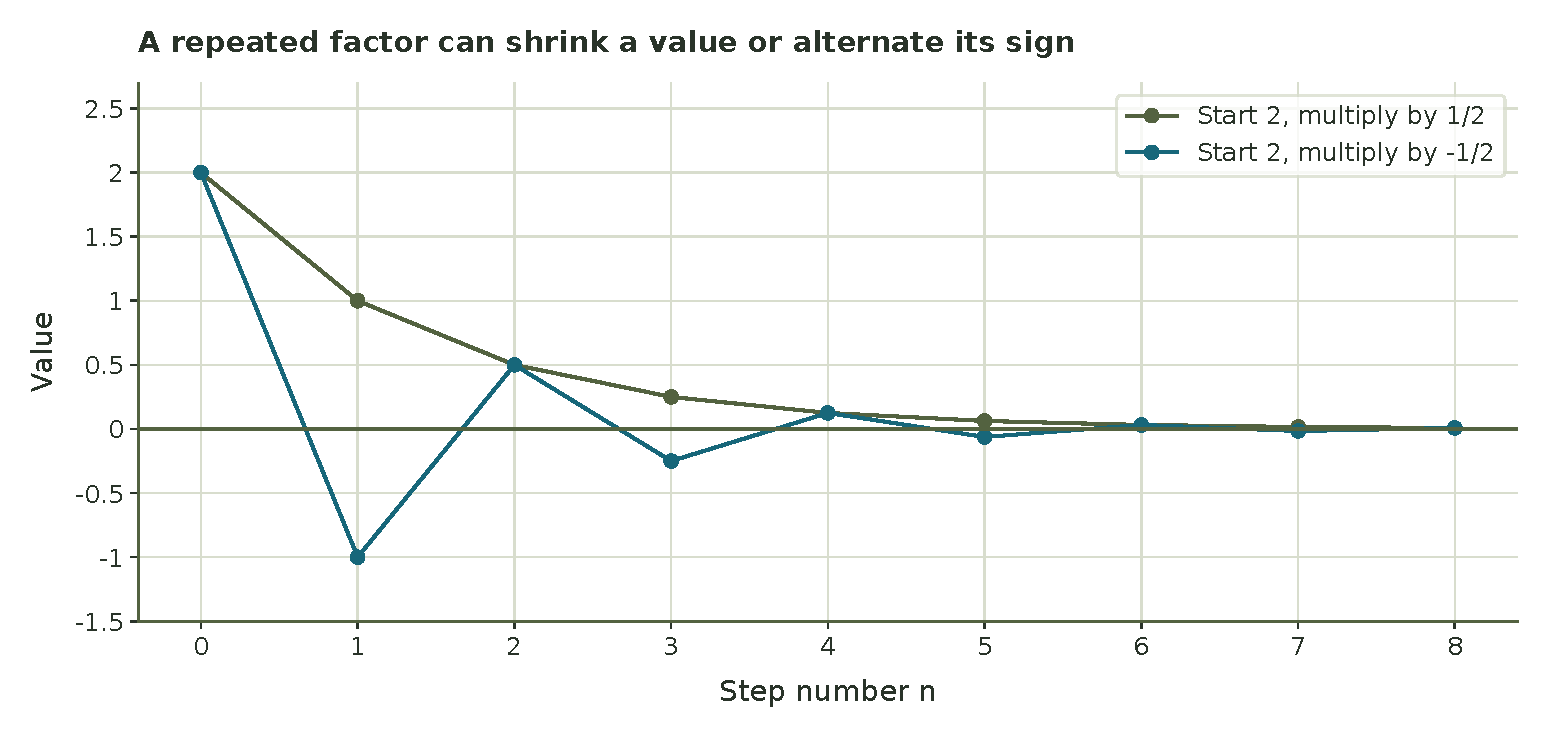
\includegraphics[width=\linewidth,height=2.65in,keepaspectratio]{../assets/week1/shrink-and-alternate.pdf}
\captionof*{figure}{The starting value and multiplier determine the pattern.}
\end{minipage}\par\medskip

With a positive start and a constant factor greater than 1, repeated multiplication eventually exceeds a fixed positive addition, if the rules continue indefinitely. A population, however, may encounter limits on space or resources.


\begin{tcolorbox}[title={When a model stops fitting},breakable,colback=warm,colbacktitle=warm,coltitle=gold,colframe=gold!35]

If a car's model value drops by 1,500 dollars every year, the arithmetic can eventually become negative. At that point, a constant annual decrease is no longer a useful model of the car's value.


\end{tcolorbox}

An additive rule changes a quantity by a fixed difference. A multiplicative rule changes it by a fixed factor. Starting from the same amount, their short-term results may be close while their longer-term results diverge.


Next week we will use fractions to describe probabilities. Later, we will revisit recursive rules when we study feedback.


\begin{tcolorbox}[title={Pause and try 13},breakable]
A model starts with 6 liters and subtracts 2 liters each day. What happens after day 3? Can the physical amount follow that rule forever?
\end{tcolorbox}

\Needspace{8\baselineskip}
\section*{More worked examples}
\subsection*{Two hypothetical balances}
Start both models at 100 dollars. A adds 20 dollars each month. B multiplies by 1.10, representing 10\% growth per month. Keep exact values while updating and round only the displayed amounts.

\par\medskip{\small\renewcommand{\arraystretch}{1.25}\begin{tabularx}{\linewidth}[t]{@{}YYY@{}}\toprule
{Month} & {A: add 20 dollars} & {B: multiply by 1.10}\\\midrule
{0} & {100.00} & {100.00}\\
{1} & {120.00} & {110.00}\\
{2} & {140.00} & {121.00}\\
{3} & {160.00} & {133.10}\\
{4} & {180.00} & {146.41}\\
{5} & {200.00} & {161.05}\\
\bottomrule\end{tabularx}}\par\medskip

\par\medskip\noindent\begin{minipage}{\linewidth}\centering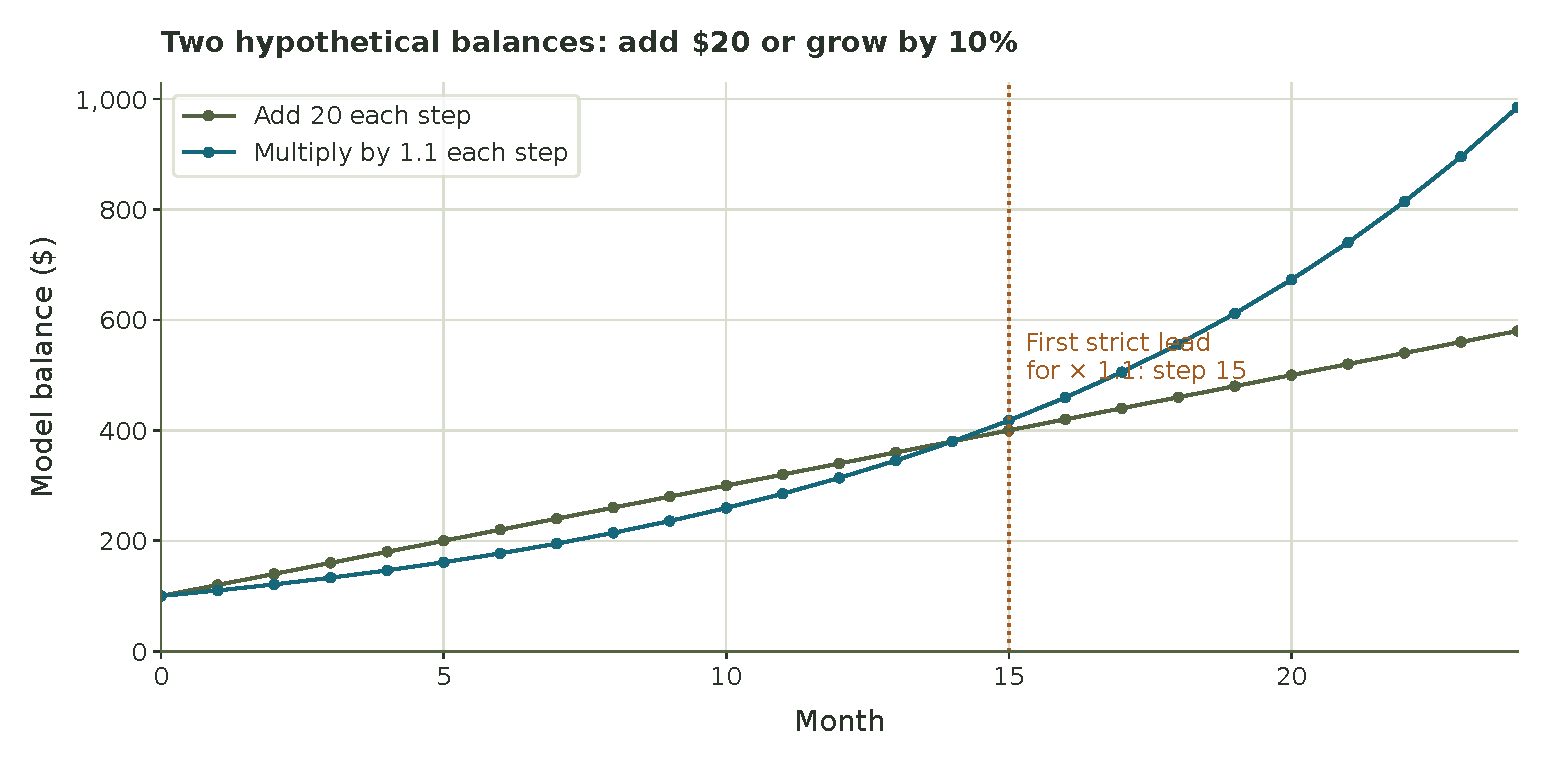
\includegraphics[width=\linewidth,height=2.65in,keepaspectratio]{../assets/week1/savings-models.pdf}\captionof*{figure}{Both rules use a positive start. The factor 1.10 exceeds 1, so the repeated multiplication eventually leads if the rules continue.}\end{minipage}\par\medskip

At month 12, A is 340.00 dollars and B is 313.84 dollars, so A still leads. At month 14, A is 380.00 and B is about 379.75. B first leads at month 15: 417.72 dollars versus A's 400.00. By month 48, the model values are 1,060.00 and 9,701.72 dollars. These are consequences of the stated update rules, not guarantees about actual accounts.

\Needspace{8\baselineskip}
\subsection*{Why the diagonal is not a fraction}
The unit-square diagonal has squared length $1^2+1^2=2$, so its exact length is $\sqrt2$. Here is a short argument that it cannot be a ratio of integers.

Suppose $\sqrt2=p/q$ in lowest terms, with positive integers p and q. Squaring gives $p^2=2q^2$. Thus $p^2$ is even, which forces p to be even: an odd number has an odd square. Write $p=2k$.

Substitution gives $4k^2=2q^2$, so $q^2=2k^2$. Then q is even too. Both p and q would share the factor 2, contradicting the assumption that the fraction was in lowest terms. This contradiction rules out a rational representation.

\Needspace{8\baselineskip}
\subsection*{Numbers that label text}
A token ID identifies a piece of text in a vocabulary. Its size does not measure meaning or dictate sentence order. In one invented vocabulary, the phrase ``cat sat on the mat'' has IDs $42,17,8,55,91$.

\par\medskip\noindent\begin{minipage}{\linewidth}\centering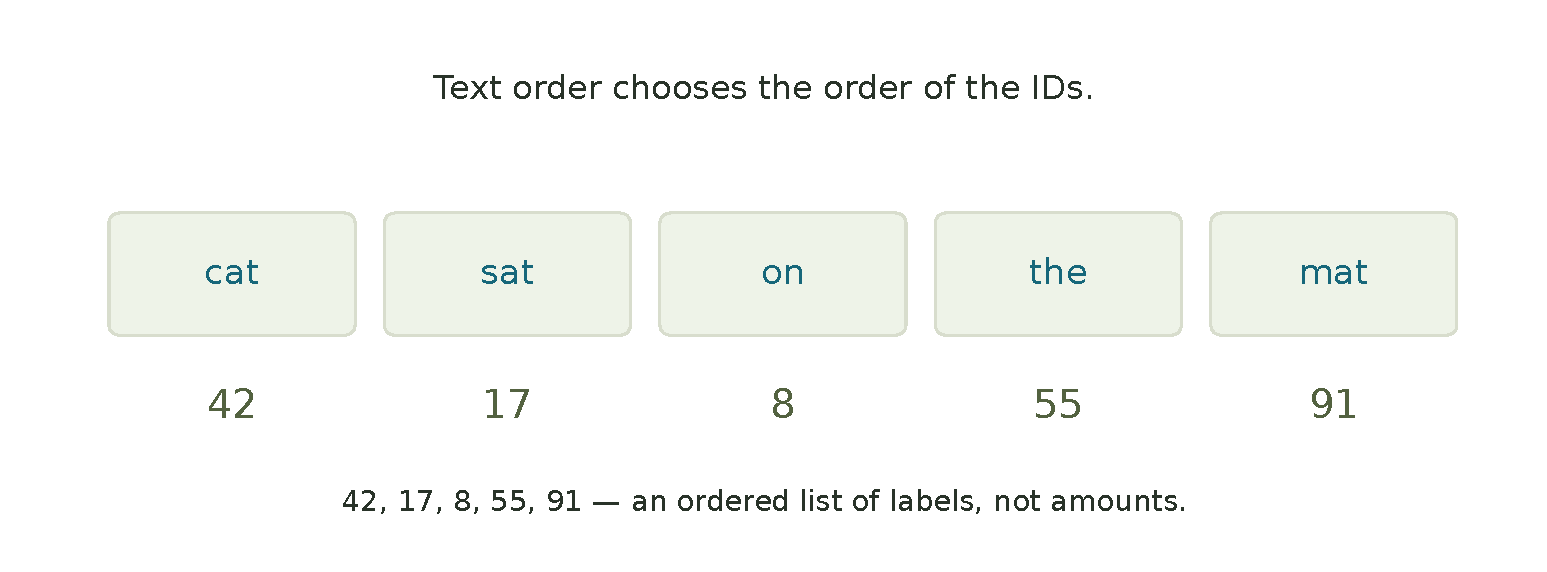
\includegraphics[width=\linewidth,height=2.65in,keepaspectratio]{../assets/week1/token-ids.pdf}\captionof*{figure}{The text gives the order of the labels. Rearranging the labels changes the text.}\end{minipage}\par\medskip

If a prompt contains 4 tokens and one token is appended per step, its length is $L_n=4+n$. The length follows an additive rule. Which token is chosen is a different question, developed through probability in Week 2.

\subsection*{Activities and further reading}
Use the \href{https://bobovski66.github.io/MathInSociety/demos/number_systems.html}{explorer} to compare sequences and fraction locations. The \href{https://bobovski66.github.io/MathInSociety/applications/week1_application.html}{growth application} compares household forecasts; the \href{https://bobovski66.github.io/MathInSociety/applications/week1_ai.html}{text-and-numbers application} distinguishes labels from quantities. The \href{https://bobovski66.github.io/MathInSociety/discussions/week1_discussion.html}{discussion} asks you to interpret a repeated change of your own.

OpenStax reviews \href{https://openstax.org/books/elementary-algebra-2e/pages/1-8-the-real-numbers}{real numbers and square roots}. Hugging Face describes \href{https://huggingface.co/docs/transformers/main_classes/tokenizer}{tokenizers and token IDs}.
\clearpage
\section*{Practice A: Number systems}
Use the smallest of N, Z, Q, and R. Here N starts at 1, and the R answer means a real number that is irrational.
\begin{enumerate}[label=A\arabic*.,leftmargin=2.5em,itemsep=10pt]
\item Classify (a) 12, (b) $-5$, (c) $3/8$, (d) $\sqrt5$, (e) 0, and (f) $6/3$.
\item Decide whether each statement is true or false and justify it in one sentence: (a) Every integer is rational. (b) Every rational number is an integer. (c) The repeating decimal $0.333\ldots=1/3$ is rational. (d) Some real numbers are not rational.
\item Write 0.75 as a simplified fraction and identify its smallest listed number system. Explain why $\sqrt3$ is not a ratio of integers.
\end{enumerate}
\Needspace{8\baselineskip}
\section*{Practice B: Addition and signed changes}
\begin{enumerate}[label=B\arabic*.,leftmargin=2.5em,itemsep=10pt]
\item Compute (a) $-8+5$, (b) $-2+(-6)$, (c) $7-(-4)$, (d) $0+(-9)$, (e) $1/4+1/4$, and (f) $2/3+1/6$.
\item A hiker starts at trail position $-6$, moves 10 units forward, then 14 backward. Write both changes as additions, give the position after each move, and mark all three positions on a number line.
\item An account starts at $-230$ dollars, receives a 500-dollar deposit, then a 185-dollar withdrawal. Write the signed additions and find the final balance.
\end{enumerate}
\Needspace{8\baselineskip}
\section*{Practice C: Multiplication and scaling}
\begin{enumerate}[label=C\arabic*.,leftmargin=2.5em,itemsep=10pt]
\item Compute (a) $(-3)7$, (b) $(-4)(-5)$, (c) $8(1/4)$, (d) $10\div(1/5)$, (e) $(2/3)(3/4)$, and (f) $(5/6)\div(1/3)$.
\item Explain in one sentence why $(-1)(-1)=1$ using reversal across zero.
\item Without first finding exact results, compare each with the positive starting value 7 and explain why: (a) $7(3/2)$, (b) $7(1/2)$, (c) $7\div(1/2)$, (d) $7\div3$.
\end{enumerate}
\Needspace{8\baselineskip}
\section*{Practice D: Rational equivalence}
\begin{enumerate}[label=D\arabic*.,leftmargin=2.5em,itemsep=10pt]
\item Test each pair for equivalence, showing cross-products: (a) $4/6$ and $6/9$, (b) $5/8$ and $15/25$, (c) $7/11$ and $21/33$, (d) $3/7$ and $9/20$.
\item Simplify (a) $12/16$, (b) $15/35$, (c) $24/36$, (d) $100/250$.
\item Simplify $0.6=6/10$, then use cross-products to verify the equivalence.
\item Explain in one sentence why $\sqrt4$ is rational while $\sqrt2$ is not.
\end{enumerate}
\Needspace{8\baselineskip}
\section*{Practice E: Operations and roots}
\begin{enumerate}[label=E\arabic*.,leftmargin=2.5em,itemsep=10pt]
\item Compute (a) $9+(-14)$, (b) $-6-(-10)$, (c) $8(3/4)$, (d) $9\div(1/3)$, (e) $7^2$, and (f) $\sqrt{144}$.
\item Identify each as rational or irrational: (a) $\sqrt{16}$, (b) $\sqrt7$, (c) $\sqrt{100}$, (d) $\sqrt{50}$.
\item A student claims $\sqrt{36}\sqrt4=\sqrt{36\cdot4}$. Check both sides, then compare $\sqrt9\sqrt9$ with $\sqrt{9\cdot9}$.
\end{enumerate}
\Needspace{8\baselineskip}
\section*{Practice F: Recursion}
Include the starting value when listing the first six terms. Label the start as step 0.
\begin{enumerate}[label=F\arabic*.,leftmargin=2.5em,itemsep=10pt]
\item List the first six terms and identify the rule type: (a) start 5, add 4; (b) start 1, multiply by 3; (c) start 100, add $-10$; (d) start 2, multiply by $1/2$.
\item A bacterial population starts at 500 and doubles every hour. Write the recursion, make a table for hours 0 through 5, and give a direct formula for hour n.
\item A car starts at 18,000 dollars and loses 1,500 dollars of model value each year. Give the first six terms. When does the model reach zero?
\item Two models start at 1,000. A adds 200 per year; B grows 15\% per year. Without calculating beyond year 5, predict which will be larger in year 20. Explain your reasoning in two sentences, assuming both rules continue.
\end{enumerate}
\Needspace{8\baselineskip}
\section*{Chapter 1 Review}
\begin{enumerate}[label=R\arabic*.,leftmargin=2.5em,itemsep=10pt]
\item Classify by the smallest listed system: (a) $8/4$, (b) $-17$, (c) $\sqrt{11}$, (d) $-6/2$.
\item A diver starts at the surface, descends 15 meters, rises 8 meters, then descends 5 meters. Write each move as a signed addition and give the final position relative to the surface.
\item Are $8/14$ and $12/21$ equivalent? Simplify both and check the cross-products.
\item A recipe uses $3/4$ cup of flour. How much is needed for $2/3$ of the recipe? Show the multiplication.
\item An insect colony starts at 80 and triples every two weeks. Give the model values at weeks 0, 2, 4, 6, and 8. Write a formula using n for the number of two-week updates, and identify the rule type.
\item A sequence is $5,5.5,6,6.5,7,\ldots$. Identify its type, give the term at step n with the start at n = 0, and find the step-20 value.
\item Compute $\sqrt{64}+3^2-((-4)\cdot2)$, showing the order of operations.
\item The diagonal of a unit square has length $\sqrt2$. Explain in two sentences why this is a real but irrational number.
\end{enumerate}

\clearpage\section*{Solutions and reasoning}

\paragraph{Short check 1.}
The route number is a label. A passenger count is a quantity. The same numeral can play either role, and the context tells us which.


\paragraph{Short check 2.}
$-$6 is an integer. 0.25 = 1/4 is rational but not an integer. 10/2 = 5 is natural. All three are also real.


\paragraph{Short check 3.}
$-$45 + 18 = $-$27 meters. The submarine is still 27 meters below the surface.


\paragraph{Short check 4.}
The change is 9 $-$ 14 = $-$5. Write 14 + ($-$5) = 9.


\paragraph{Short check 5.}
Both simplify to 3/5. Their cross-products also agree: 6 $\times$ 15 = 90 and 10 $\times$ 9 = 90.


\paragraph{Short check 6.}
The sum is 2/4 + 1/4 = 3/4. The product is 1/8: one half of one fourth. Combining two amounts and taking a fraction of an amount are different operations.


\paragraph{Short check 7.}
Multiplying by 1/3 gives less than 9. Dividing by 1/3 is multiplying by 3, giving more than 9.


\paragraph{Short check 8.}
The factor is 1.25. The new quantity is 80 $\times$ 1.25 = 100. The increase itself is 20.


\paragraph{Short check 9.}
Both distributive expressions give 21. The squared quantity is ($-$3)$^2$ = 9, so its nonnegative square root is 3.


\paragraph{Short check 10.}
\(\sqrt{25}\) = 5 is rational. \(\sqrt{6}\) is irrational because 6 is a nonnegative integer that is not a perfect square. The finite decimal 2.44949 is rational, even if it is being used to approximate \(\sqrt{6}\).


\paragraph{Short check 11.}
The real part is 5 and the imaginary part is $-$2. Its point is (5,$-$2).


\paragraph{Short check 12.}
The list is 9, 7, 5, 3, 1. The step-4 value is 1. The starting value and four updates give five terms.


\paragraph{Short check 13.}
The model values at days 0 through 3 are 6, 4, 2, and 0 liters. Continuing the arithmetic would give negative amounts. An actual stored amount cannot keep following that rule after the supply is exhausted.


\Needspace{8\baselineskip}

\Needspace{8\baselineskip}\subsection*{Practice A: Number systems}
\begin{enumerate}[label=A\arabic*.,leftmargin=2.5em,itemsep=10pt]
\item (a) N. (b) Z. (c) Q. (d) R, real but irrational. (e) Z under the four listed choices. (f) $6/3=2$, so N. Every one is also real; the task asks for the smallest listed system.
\item (a) True: any integer k equals $k/1$. (b) False: $1/2$ is rational but not an integer. (c) True: $1/3$ is a ratio of integers. (d) True: $\sqrt2$ is one example.
\item $0.75=75/100=3/4$, so its smallest listed system is Q. The square root of a nonnegative integer that is not a perfect square is irrational; 3 is such an integer, so $\sqrt3$ is not a ratio of integers.
\end{enumerate}

\Needspace{8\baselineskip}\subsection*{Practice B: Signed changes}
\begin{enumerate}[label=B\arabic*.,leftmargin=2.5em,itemsep=10pt]
\item (a) $-3$. (b) $-8$. (c) $11$. (d) $-9$. (e) $1/2$. (f) $2/3+1/6=4/6+1/6=5/6$.
\item The signed updates are $-6+10=4$, followed by $4+(-14)=-10$. On a number line, mark $-6$, 4, and $-10$, with the first move right and the second left.
\par\medskip\noindent\begin{minipage}{\linewidth}\centering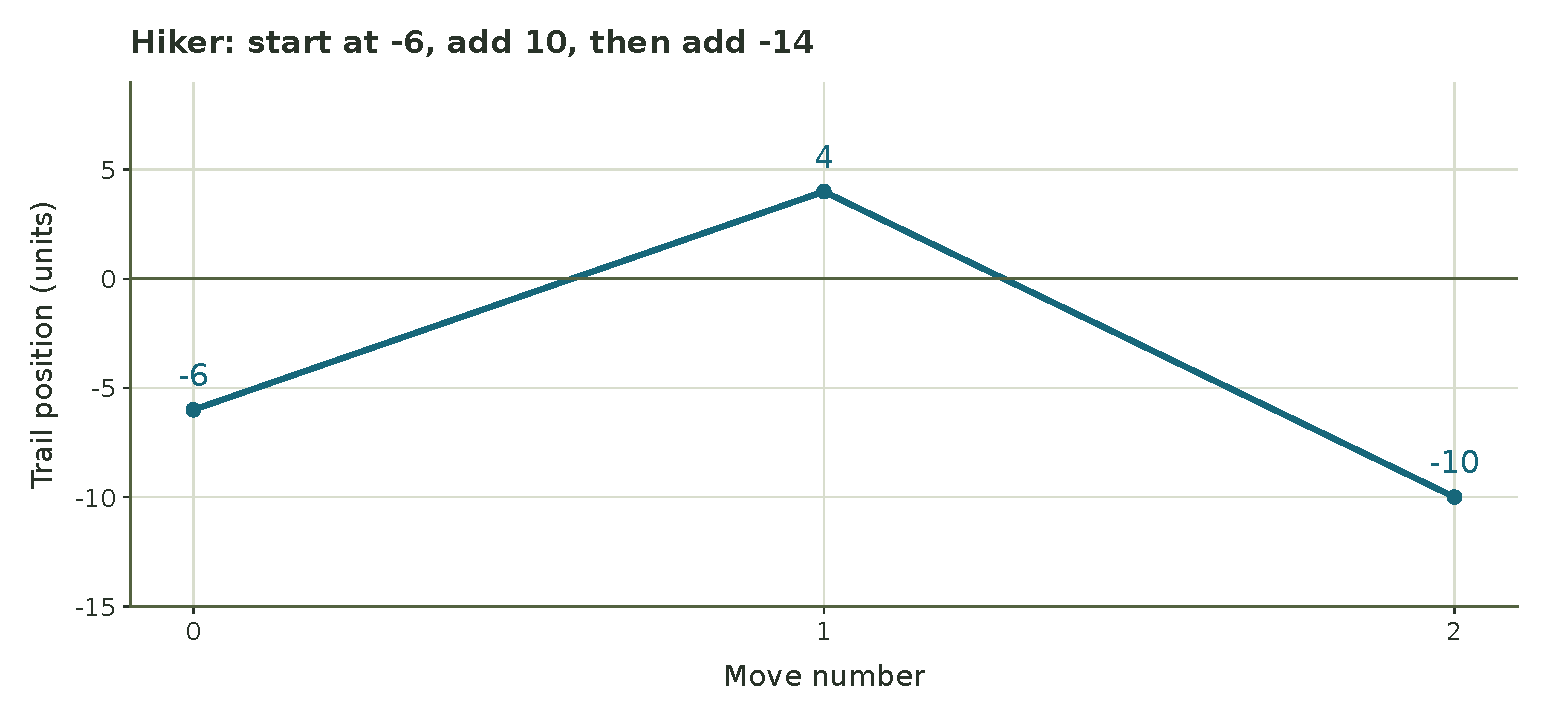
\includegraphics[width=\linewidth,height=2.65in,keepaspectratio]{../assets/week1/hiker-path.pdf}\captionof*{figure}{The graph records position after each move. The three marked values are the locations to place on a number line.}\end{minipage}\par\medskip

\item $-230+500+(-185)=270-185=85$. The final balance is 85 dollars. The deposit is positive and the withdrawal is negative.
\end{enumerate}

\Needspace{8\baselineskip}\subsection*{Practice C: Scaling}
\begin{enumerate}[label=C\arabic*.,leftmargin=2.5em,itemsep=10pt]
\item (a) $-21$. (b) 20. (c) 2. (d) $10(5)=50$. (e) $6/12=1/2$. (f) $(5/6)(3)=15/6=5/2$.
\item Multiplication by $-1$ reverses direction across zero, so doing it twice returns to the original positive unit.
\item (a) Greater: the factor $3/2$ exceeds 1. (b) Less: the factor $1/2$ lies between 0 and 1. (c) Greater: division by $1/2$ multiplies by 2. (d) Less: division by 3 multiplies by $1/3$. These comparisons use a positive starting value.
\end{enumerate}

\Needspace{8\baselineskip}\subsection*{Practice D: Equivalence}
\begin{enumerate}[label=D\arabic*.,leftmargin=2.5em,itemsep=10pt]
\item (a) Equivalent: $4(9)=6(6)=36$. (b) Different: $5(25)=125$ and $8(15)=120$. (c) Equivalent: $7(33)=11(21)=231$. (d) Different: $3(20)=60$ and $7(9)=63$.
\item (a) $3/4$ after dividing by 4. (b) $3/7$ after dividing by 5. (c) $2/3$ after dividing by 12. (d) $2/5$ after dividing by 50.
\item $6/10=3/5$ after dividing numerator and denominator by 2. The cross-products agree: $6(5)=10(3)=30$.
\item $\sqrt4=2=2/1$ is rational, whereas $\sqrt2$ cannot be written as a ratio of integers, as the lowest-terms argument in the worked examples shows.
\end{enumerate}

\Needspace{8\baselineskip}\subsection*{Practice E: Operations and roots}
\begin{enumerate}[label=E\arabic*.,leftmargin=2.5em,itemsep=10pt]
\item (a) $-5$. (b) 4. (c) 6. (d) 27. (e) 49. (f) 12.
\item (a) $\sqrt{16}=4$, rational. (b) $\sqrt7$, irrational. (c) $\sqrt{100}=10$, rational. (d) $\sqrt{50}$, irrational because the nonnegative integer 50 is not a perfect square. It also equals $5\sqrt2$.
\item The first left side is $6(2)=12$; the right side is $\sqrt{144}=12$. In the second check, $\sqrt9\sqrt9=3(3)=9$ and $\sqrt{9\cdot9}=\sqrt{81}=9$. Products of principal square roots obey this rule for nonnegative real quantities under the roots.
\end{enumerate}

\Needspace{8\baselineskip}\subsection*{Practice F: Recursion}
\begin{enumerate}[label=F\arabic*.,leftmargin=2.5em,itemsep=10pt]
\item (a) $5,9,13,17,21,25$, additive.\par (b) $1,3,9,27,81,243$, multiplicative.\par (c) $100,90,80,70,60,50$, additive with change $-10$.\par (d) $2,1,1/2,1/4,1/8,1/16$, multiplicative with factor $1/2$.\par Six terms include the start and five updates.
\item $b_0=500$ and $b_{n+1}=2b_n$. The direct formula is $b_n=500(2^n)$.
\par\medskip{\small\renewcommand{\arraystretch}{1.25}\begin{tabularx}{\linewidth}[t]{@{}YY@{}}\toprule
{Hour n} & {Model population}\\\midrule
{0} & {500}\\
{1} & {1000}\\
{2} & {2000}\\
{3} & {4000}\\
{4} & {8000}\\
{5} & {16000}\\
\bottomrule\end{tabularx}}\par\medskip
The doubled counts follow the mathematical rule; an actual culture can encounter limits.
\item The first six values are $18{,}000,16{,}500,15{,}000,13{,}500,12{,}000,10{,}500$ dollars. Solve $18{,}000-1{,}500n=0$ to obtain $n=12$ years.
\par\medskip\noindent\begin{minipage}{\linewidth}\centering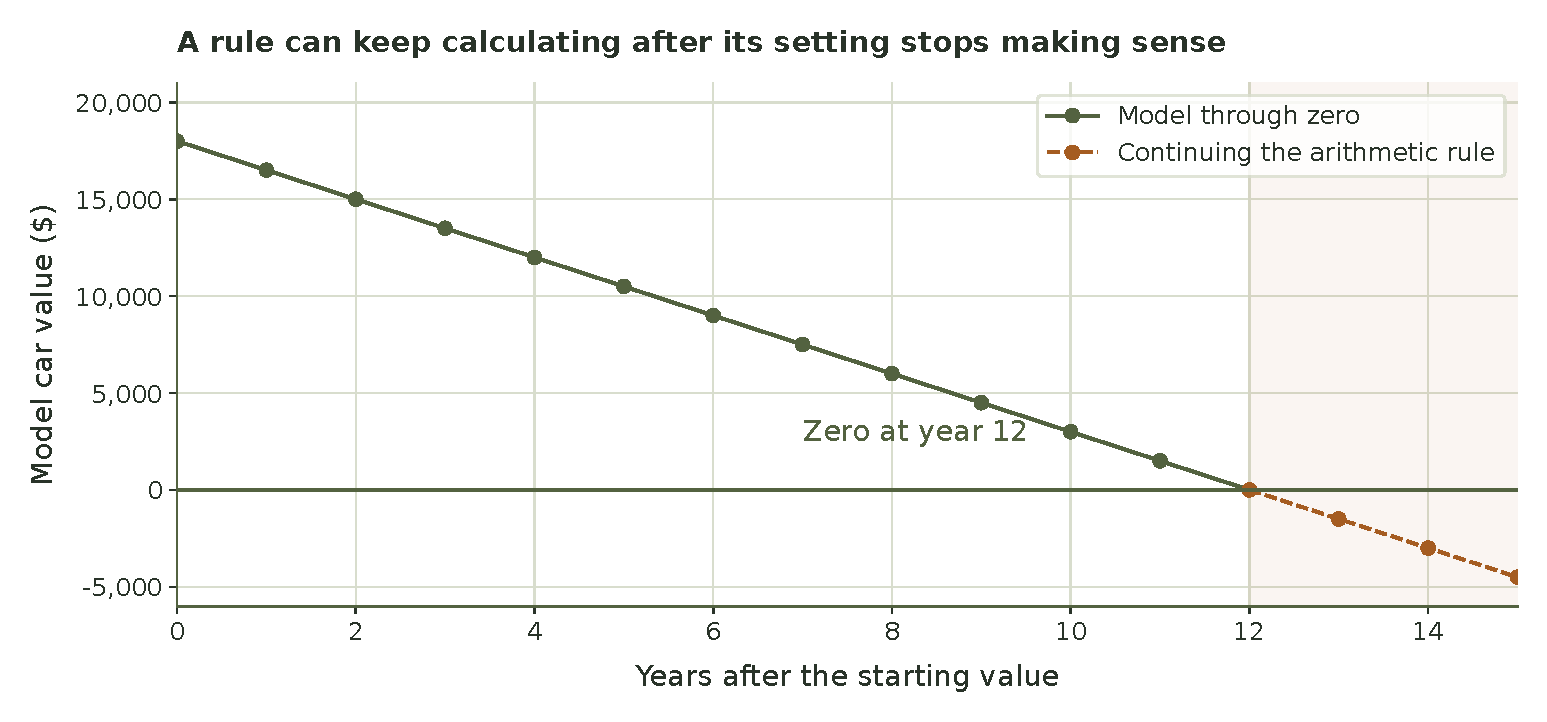
\includegraphics[width=\linewidth,height=2.65in,keepaspectratio]{../assets/week1/car-value.pdf}\captionof*{figure}{The arithmetic becomes negative after year 12. That extension shows where the rule needs reconsideration as a model of car value.}\end{minipage}\par\medskip

\item Predict B. By year 5, B is about 2,011.36 while A is 2,000, and B is already gaining more than 200 per year; its annual gain continues to increase under the fixed 15\% rule, so it remains ahead through year 20 if the rules continue.
\par\medskip{\small\renewcommand{\arraystretch}{1.25}\begin{tabularx}{\linewidth}[t]{@{}YYY@{}}\toprule
{Year} & {A: add 200} & {B: multiply by 1.15}\\\midrule
{0} & {1000} & {1,000.00}\\
{1} & {1200} & {1,150.00}\\
{2} & {1400} & {1,322.50}\\
{3} & {1600} & {1,520.88}\\
{4} & {1800} & {1,749.01}\\
{5} & {2000} & {2,011.36}\\
\bottomrule\end{tabularx}}\par\medskip

\par\medskip\noindent\begin{minipage}{\linewidth}\centering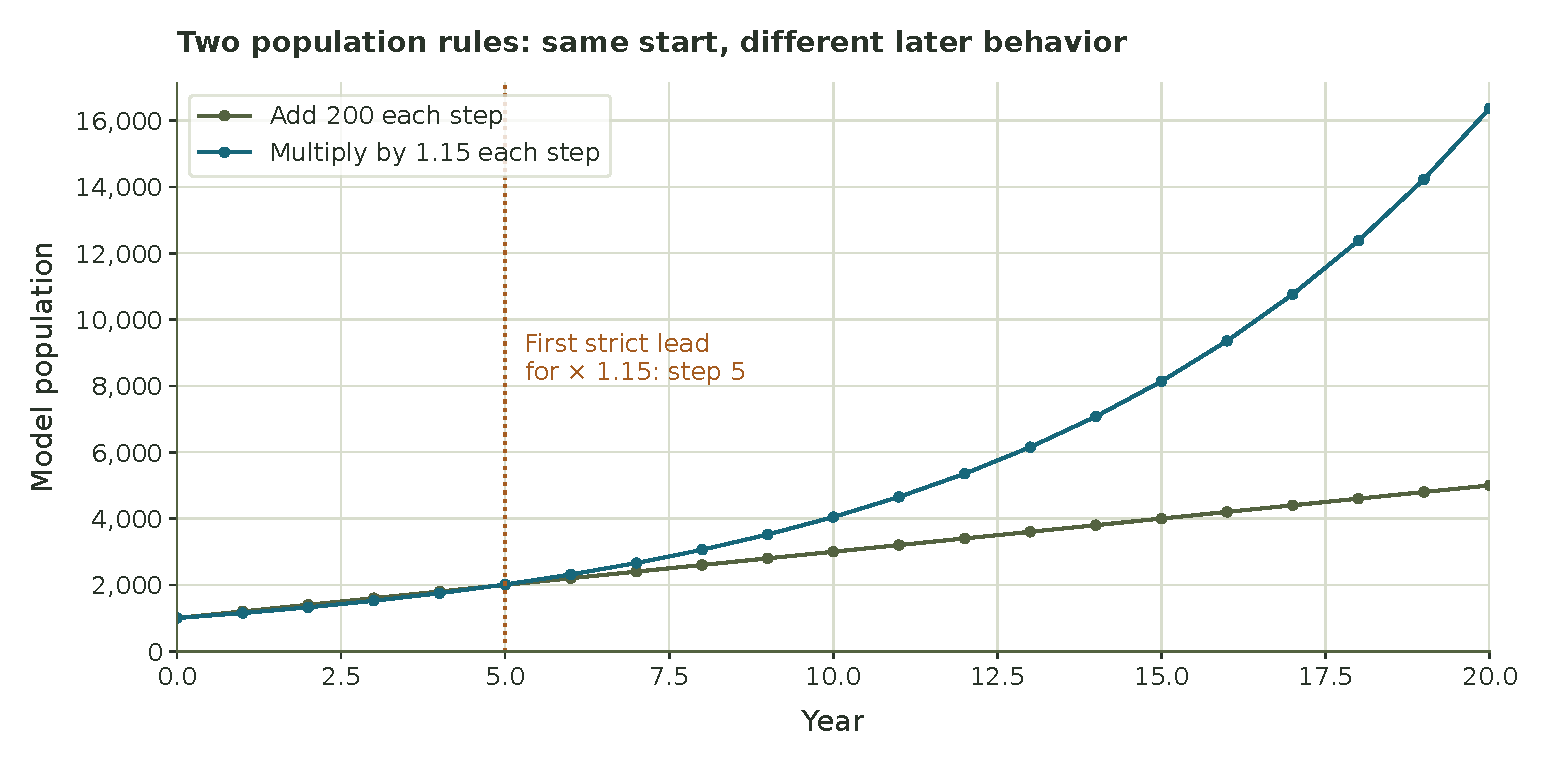
\includegraphics[width=\linewidth,height=2.65in,keepaspectratio]{../assets/week1/recursion-comparison.pdf}\captionof*{figure}{A numerical check at year 20 gives A = 5,000 and B approximately 16,366.54. The prediction above uses only the behavior through year 5.}\end{minipage}\par\medskip

\end{enumerate}

\Needspace{8\baselineskip}\subsection*{Chapter 1 review}
\begin{enumerate}[label=R\arabic*.,leftmargin=2.5em,itemsep=10pt]
\item (a) $8/4=2$: N. (b) $-17$: Z. (c) $\sqrt{11}$: R, real but irrational. (d) $-6/2=-3$: Z.
\item $0+(-15)=-15$, then $-15+8=-7$, then $-7+(-5)=-12$. The final position is $-12$ meters relative to the surface: the diver is 12 meters below it.
\par\medskip\noindent\begin{minipage}{\linewidth}\centering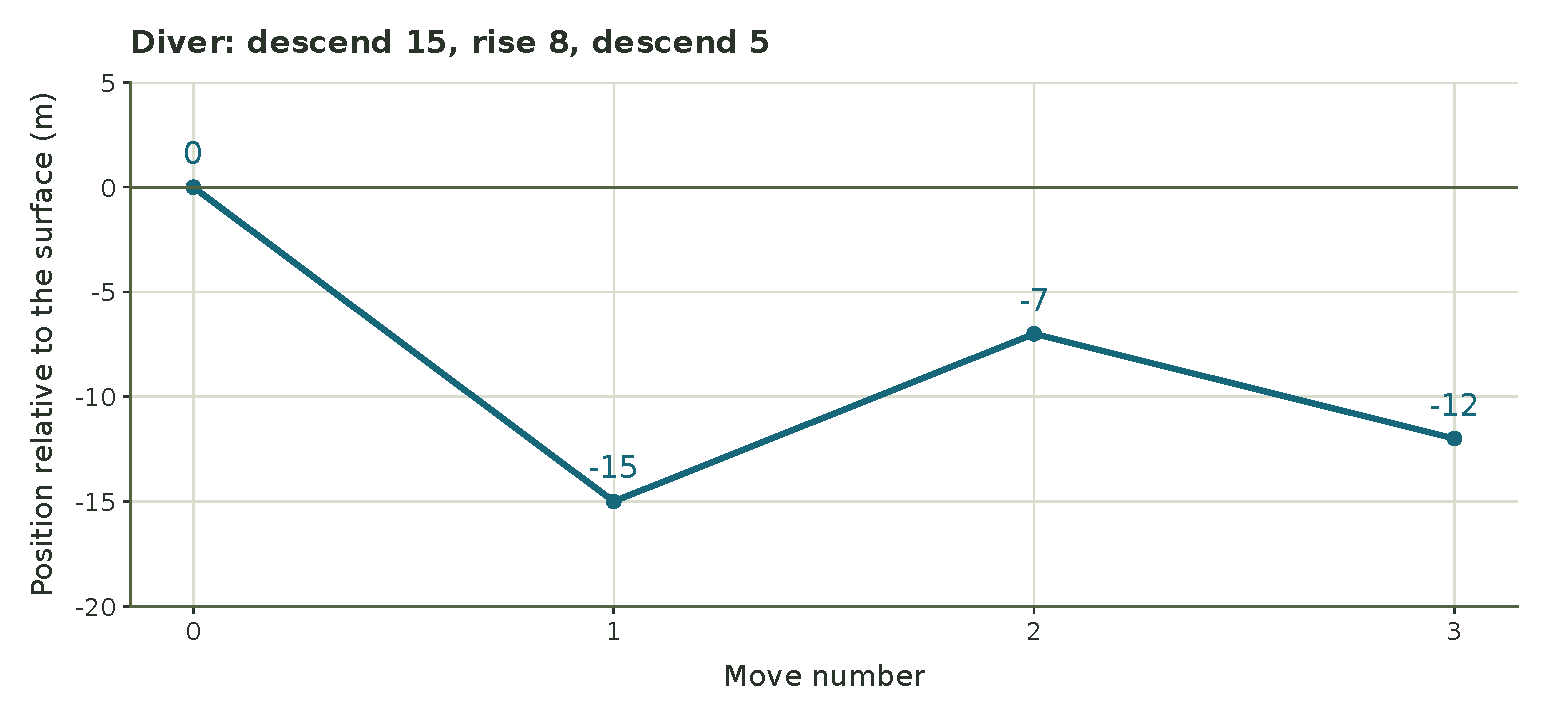
\includegraphics[width=\linewidth,height=2.65in,keepaspectratio]{../assets/week1/diver-path.pdf}\captionof*{figure}{Signed position and depth below the surface use different descriptions of the same stop.}\end{minipage}\par\medskip

\item Both simplify to $4/7$: divide $8/14$ by 2 and $12/21$ by 3. The original cross-products agree: $8(21)=14(12)=168$.
\item $(2/3)(3/4)=6/12=1/2$ cup.
\par\medskip\noindent\begin{minipage}{\linewidth}\centering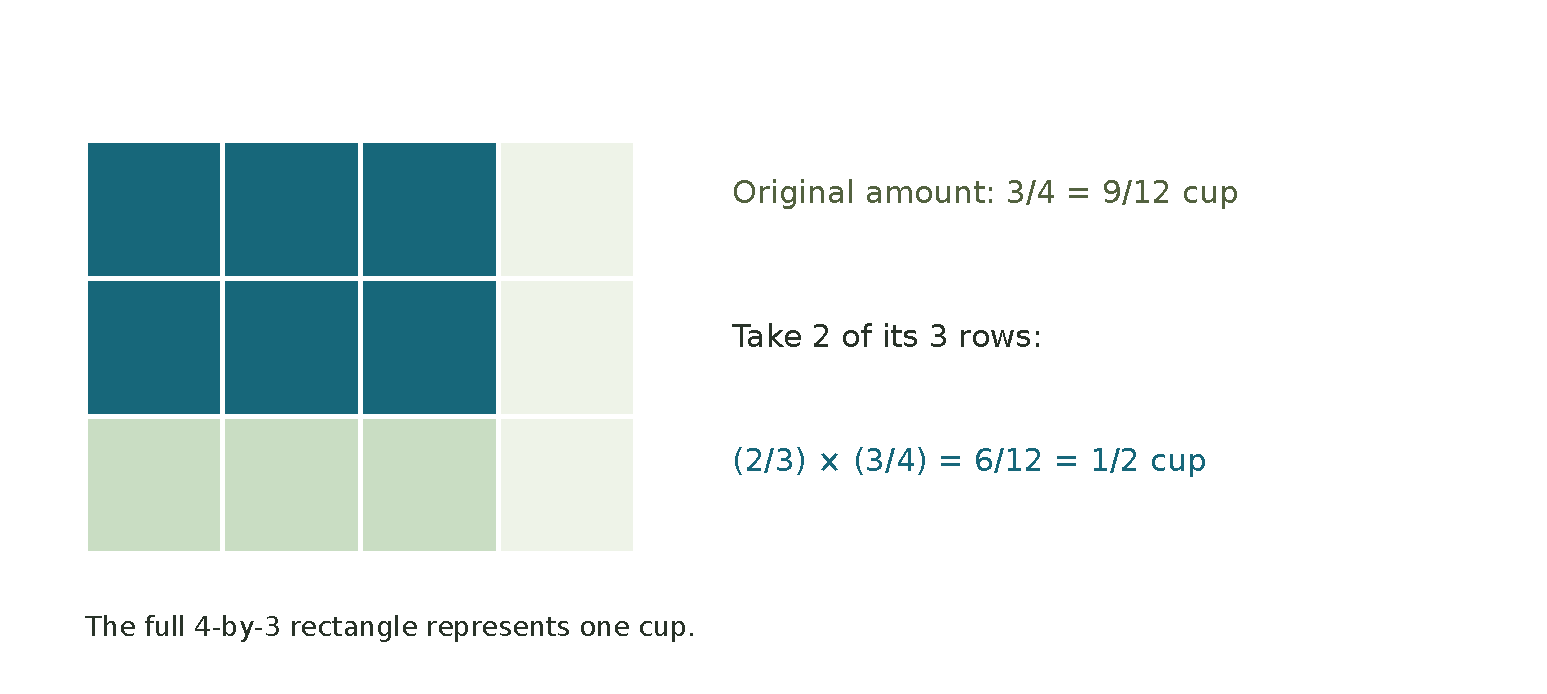
\includegraphics[width=\linewidth,height=2.65in,keepaspectratio]{../assets/week1/fraction-scale.pdf}\captionof*{figure}{Two thirds of the original three-quarter cup is half a cup.}\end{minipage}\par\medskip

\item
\par\medskip{\small\renewcommand{\arraystretch}{1.25}\begin{tabularx}{\linewidth}[t]{@{}YYY@{}}\toprule
{Weeks} & {Two-week updates n} & {Model insects}\\\midrule
{0} & {0} & {80}\\
{2} & {1} & {240}\\
{4} & {2} & {720}\\
{6} & {3} & {2160}\\
{8} & {4} & {6480}\\
\bottomrule\end{tabularx}}\par\medskip
The direct formula is $P_n=80(3^n)$, with one update every two weeks. This is multiplicative recursion; n is not the number of individual weeks.
\par\medskip\noindent\begin{minipage}{\linewidth}\centering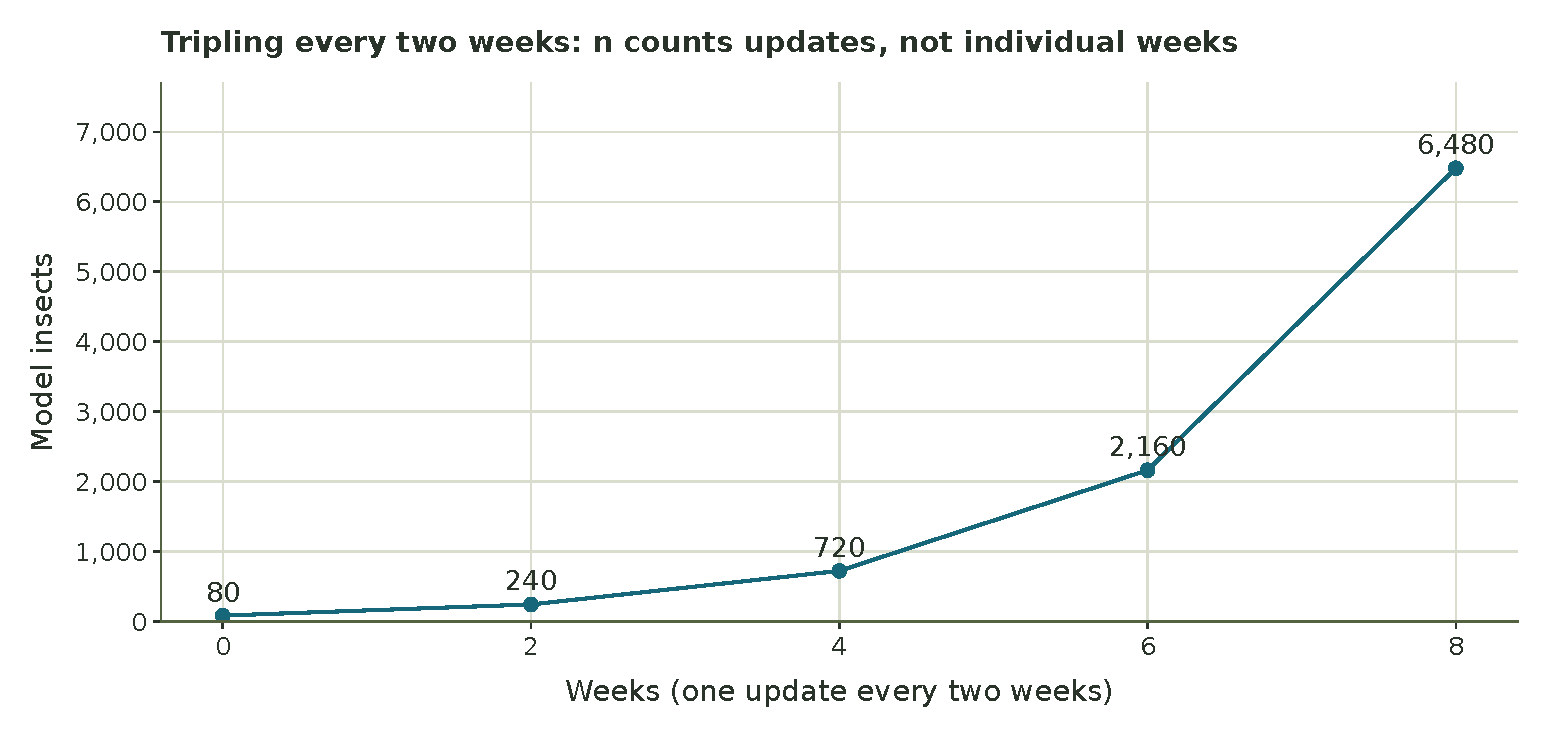
\includegraphics[width=\linewidth,height=2.65in,keepaspectratio]{../assets/week1/insect-growth.pdf}\captionof*{figure}{The update interval must match the exponent in the model.}\end{minipage}\par\medskip

\item This is additive with change 0.5: $a_n=5+0.5n$. At step 20, $a_{20}=5+0.5(20)=15$.
\item First take the square root and square: $8+9-((-4)\cdot2)$. Multiply inside the parentheses to get $8+9-(-8)$, then add the opposite: $8+9+8=25$.
\item The unit-square diagonal has a real length whose square is 2. If that length were a reduced fraction $p/q$, then $p^2=2q^2$ would force both p and q to be even, contradicting lowest terms, so the length is irrational.
\end{enumerate}

\end{document}
